\documentclass[11pt,a4paper]{article}

% Packages
% NOTE: the legacy vietnam+babel[vietnamese] combo (T5-encoded 8-bit fonts)
% renders Vietnamese diacritics incorrectly under this tectonic build (silent
% wrong-glyph substitution, not just missing-character warnings). Tectonic's
% engine is XeTeX-based, so fontspec + a Unicode font bypasses that broken
% legacy path entirely and renders correctly.
\usepackage{fontspec}

\setmainfont{Times New Roman}
\setsansfont{Arial}
\setmonofont{Consolas}
\usepackage[x11names,rgb]{xcolor}
\usepackage{amsmath,amssymb,amsthm}
\usepackage{graphicx}
\usepackage{tikz}
\usepackage{multirow}
\usetikzlibrary{shapes.geometric,arrows,positioning,calc,
                decorations.pathreplacing,fit,backgrounds,arrows.meta}
\usepackage{listings}
\usepackage{hyperref}
\usepackage{geometry}
\usepackage{fancyhdr}
\usepackage{tocloft}
\usepackage{caption}
\usepackage{subcaption}
\usepackage{stmaryrd}
\usepackage{mathtools}
\usepackage{tcolorbox}
\tcbuselibrary{skins,breakable}
\usepackage{proof}
\usepackage{subcaption}
\usepackage{amsfonts}
\usepackage{amsmath,amssymb,amsthm}
\usepackage{tcolorbox}
\usepackage{float}
\usepackage{indentfirst}
\usepackage{booktabs}
\usepackage{titlesec}
\usepackage{lastpage}

% --- ALGORITHM PACKAGES ---
% Use 'algorithm' for the float wrapper and 'algpseudocode' for the syntax.
% Do NOT load 'algorithmic'.
\usepackage{algorithm}
\usepackage{algpseudocode}

% --- CUSTOMIZATION ---
\algrenewcommand{\algorithmicrequire}{\textbf{Input:}}
\algrenewcommand{\algorithmicensure}{\textbf{Output:}}
\algrenewcommand{\algorithmiccomment}[1]{\hfill\textcolor{gray}{\textit{\{#1\}}}}

\newtheorem{definition}{Định nghĩa}
\newtheorem{example}{Ví dụ}
\newtheorem{remark}{Nhận xét}

% Marker for sections of the outline that still need real content/data filled in.
\newcommand{\TODO}[1]{\textcolor{red!70!black}{\textbf{[TODO: #1]}}}

% Page layout
\geometry{left=2cm,right=2cm,top=2.8cm,bottom=2.4cm,headheight=32pt,headsep=0.45cm,footskip=1.1cm}
\setlength{\emergencystretch}{2em}

% Cho phép ngắt dòng sau dấu gạch dưới trong \texttt{...}
\let\originalunderscore\_
\renewcommand{\_}{\originalunderscore\allowbreak}

% Header/Footer
\pagestyle{fancy}
\fancyhf{}
\fancyhead[L]{%
    \begin{minipage}[c]{0.075\textwidth}
        
\includegraphics[width=0.72cm]{figs/HCMUT.pdf}
    \end{minipage}%
    \begin{minipage}[c]{0.79\textwidth}
        \small Trường Đại học Bách khoa, ĐHQG TP. Hồ Chí Minh\\[-1pt]
        \small Khoa Khoa học và Kỹ thuật Máy tính
    \end{minipage}}
\renewcommand{\headrulewidth}{0.4pt}
\fancyfoot[L]{\footnotesize Báo cáo Đồ án -- P4AIDS}
\fancyfoot[R]{\footnotesize Page \thepage/\pageref{LastPage}}
\renewcommand{\footrulewidth}{0.4pt}

\fancypagestyle{plain}{%
    \fancyhf{}
    \fancyhead[L]{%
        \begin{minipage}[c]{0.075\textwidth}
            
\includegraphics[width=0.72cm]{figs/HCMUT.pdf}
        \end{minipage}%
        \begin{minipage}[c]{0.79\textwidth}
            \small Trường Đại học Bách khoa, ĐHQG TP. Hồ Chí Minh\\[-1pt]
            \small Khoa Khoa học và Kỹ thuật Máy tính
        \end{minipage}}
    \fancyfoot[L]{\footnotesize Báo cáo Đồ án -- P4AIDS}
    \fancyfoot[R]{\footnotesize Page \thepage/\pageref{LastPage}}
    \renewcommand{\headrulewidth}{0.4pt}
    \renewcommand{\footrulewidth}{0.4pt}
}

% Chapter-like section headings while retaining the article class
\titleformat{\section}[display]
  {\normalfont\bfseries}
  {\fontsize{26}{31}\selectfont\thesection}
  {0.35em}
  {\fontsize{22}{27}\selectfont\raggedright}
\titlespacing*{\section}{0pt}{0.45cm}{1.1cm}

\titleformat{\subsection}
  {\normalfont\Large\bfseries}
  {\thesubsection}{0.7em}{}
\titleformat{\subsubsection}
  {\normalfont\normalsize\bfseries}
  {\thesubsubsection}{0.7em}{}
\titleformat{\paragraph}[runin]
  {\normalfont\normalsize\bfseries\itshape}
  {}{0pt}{}
\titlespacing*{\paragraph}{0pt}{0.35cm}{0.6em}

% Table of contents and list of figures
\renewcommand{\contentsname}{Mục lục}
\renewcommand{\listfigurename}{Danh sách hình ảnh}
\renewcommand{\listtablename}{Danh sách bảng}
\renewcommand{\cfttoctitlefont}{\Large\bfseries}
\renewcommand{\cftloftitlefont}{\Large\bfseries}
\renewcommand{\cftlottitlefont}{\Large\bfseries}
\renewcommand{\cftsecfont}{\bfseries}
\renewcommand{\cftsecpagefont}{\bfseries}
\setlength{\cftbeforesecskip}{0.45em}

% Code listing style
\definecolor{codegreen}{rgb}{0,0.6,0}
\definecolor{codegray}{rgb}{0.5,0.5,0.5}
\definecolor{codepurple}{rgb}{0.58,0,0.82}
\definecolor{backcolour}{rgb}{0.95,0.95,0.92}

\lstdefinestyle{mystyle}{
    backgroundcolor=\color{backcolour},
    commentstyle=\color{codegreen},
    keywordstyle=\color{magenta},
    numberstyle=\tiny\color{codegray},
    stringstyle=\color{codepurple},
    basicstyle=\ttfamily\footnotesize,
    breakatwhitespace=false,
    breaklines=true,
    captionpos=b,
    keepspaces=true,
    numbers=left,
    numbersep=5pt,
    showspaces=false,
    showstringspaces=false,
    showtabs=false,
    tabsize=2
}

\lstset{style=mystyle}

% Hyperref setup
\hypersetup{
    colorlinks=true,
    linkcolor=black,
    filecolor=magenta,
    citecolor=black,
    urlcolor=blue,
    pdftitle={bao_cao_rain_snow_classification},
}

% TikZ styles
\tikzset{
    process/.style={rectangle, minimum width=2.5cm, minimum height=1cm,
                   text centered, draw=black, fill=blue!20},
    server/.style={cylinder, shape border rotate=90, minimum width=2cm,
                  minimum height=1.5cm, draw=black, fill=green!20},
    client/.style={rectangle, rounded corners, minimum width=2cm,
                  minimum height=1cm, draw=black, fill=orange!20},
    arrow/.style={thick,->,>=stealth},
    bidiarrow/.style={thick,<->,>=stealth},
}

\begin{document}

% Title page
\begin{titlepage}
    \thispagestyle{empty}
    \begin{tikzpicture}[remember picture,overlay]
        \draw[line width=0.8pt]
            ($(current page.north west)+(0.8cm,-0.8cm)$)
            rectangle
            ($(current page.south east)+(-0.8cm,0.8cm)$);
        \draw[line width=0.35pt]
            ($(current page.north west)+(1.05cm,-1.05cm)$)
            rectangle
            ($(current page.south east)+(-1.05cm,1.05cm)$);
        \draw[line width=0.35pt]
            ($(current page.north west)+(1.28cm,-0.68cm)$) --
            ($(current page.north east)+(-1.28cm,-0.68cm)$);
        \draw[line width=0.35pt]
            ($(current page.south west)+(1.28cm,0.68cm)$) --
            ($(current page.south east)+(-1.28cm,0.68cm)$);
    \end{tikzpicture}
    \centering
    \vspace*{0.55cm}

    {\Large\textbf{ĐẠI HỌC QUỐC GIA TP.HỒ CHÍ MINH}}\\[0.3cm]
    {\Large\textbf{TRƯỜNG ĐẠI HỌC BÁCH KHOA}}\\[0.3cm]
    {\large KHOA KHOA HỌC VÀ KỸ THUẬT MÁY TÍNH}\\[2cm]

    
\includegraphics[width=0.3\textwidth]{figs/HCMUT.pdf}\\[1cm]

    {\large\textbf{BÁO CÁO BÀI TẬP LỚN }}\\
    {\Large\textbf{LẬP TRÌNH CHO TRÍ TUỆ NHÂN TẠO VÀ KHOA HỌC DỮ LIỆU}}\\[0.5cm]
    {\LARGE\textbf{
        PHÂN LOẠI PHA GIÁNG THỦY MƯA/TUYẾT TỪ DỮ LIỆU THỜI TIẾT SZEGED
        KHI CẢM BIẾN BỊ MẤT SỐ ĐO: SO SÁNH HỌC MÁY CỔ ĐIỂN, ROCKET
        VÀ HỌC SÂU CHO DỮ LIỆU CHUỖI THỜI GIAN THIẾU
    }}\\[0.3cm]
    {\small\itshape
        Rain/Snow Phase Classification on the Szeged Weather Dataset under
        Sensor Missingness: Benchmarking Classic ML, ROCKET and Deep Learning
        for Incomplete Time Series
    }\\[0.3cm]

    \vfill

    \begin{tabular}{@{}r l@{}}
        \textbf{Sinh viên thực hiện:}   & \TODO{Họ và tên} -- \TODO{MSSV}\\
                                        & \TODO{Họ và tên} -- \TODO{MSSV}\\
                                        & \TODO{Họ và tên} -- \TODO{MSSV}\\
                                        & \TODO{Họ và tên} -- \TODO{MSSV}\\
                                        & \TODO{Họ và tên} -- \TODO{MSSV}\\[0.35cm]
        \textbf{Giảng viên hướng dẫn:}  & \TODO{Họ và tên GVHD}
    \end{tabular}

    \vfill

    {\large \textit{TP. Hồ Chí Minh, tháng \number\month{} năm \number\year}}
\end{titlepage}

% Table of contents
\pagenumbering{Roman}
\tableofcontents
\newpage
\addcontentsline{toc}{section}{Danh sách hình ảnh}
\listoffigures
\newpage
\addcontentsline{toc}{section}{Danh sách bảng}
\listoftables
\newpage
\pagenumbering{arabic}
\setcounter{page}{1}

% Abstract / Tóm tắt
\section*{Tóm tắt}
\addcontentsline{toc}{section}{Tóm tắt}

Phân biệt mưa và tuyết tại thời điểm $t+1$ là một bài toán phân loại thời tiết quan
trọng cho cảnh báo giao thông, nông nghiệp và vận hành lưới điện, nhưng các trạm quan
trắc thực tế thường xuyên mất số đo do lỗi cảm biến, mất điện hoặc lỗi truyền tín hiệu.
Đồ án này xây dựng và đánh giá một benchmark trên bộ dữ liệu thời tiết Szeged
(2006--2016), với đầu vào là cửa sổ trượt 24 giờ của 5 biến quan trắc (nhiệt độ, độ ẩm,
tốc độ gió, áp suất, tầm nhìn) và đầu ra là nhãn Rain/Snow tại
$t+1$, trong điều kiện dữ liệu bị thiếu được giả lập theo ba kiểu (điểm, đoạn liên tiếp,
khối) ở các tỷ lệ 10/30/50\%.

Benchmark được thiết kế cho ba hướng phương pháp: học máy cổ điển dựa trên
đặc trưng chuỗi thời gian, họ biến đổi ROCKET và học sâu xử lý dữ liệu thiếu.
Bộ kết quả hiện có hoàn tất 150 lượt của năm mô hình DL: GRU-Fill,
GRU+mask/$\Delta t$, GRU-D tự cài, BRITS và SAITS, trên cùng tập chia thời gian
và bộ mask, với ba seed huấn luyện.

Trên chín điều kiện thiếu, SAITS có Macro F1 trung bình cao nhất (0.91418),
còn BRITS đứng đầu tại point 50\% (0.9281) và subsequence 50\% (0.8682).
Bổ sung mask/$\Delta t$ cải thiện GRU-Fill ở bảy trong chín điều kiện.
SAITS dùng khoảng 126.17 phút cho 30 lượt, so với 1255.97 phút của BRITS;
đây là thời gian toàn pipeline, không phải train hoặc inference thuần.
Cả năm mô hình có Macro F1 thấp nhất ở subsequence 50\%.
Chưa có kết quả ML/ROCKET trong bộ phân tích, chưa kiểm định ý nghĩa thống kê
và chưa thực hiện SHAP/Integrated Gradients; UniTS là hướng mở rộng chưa triển khai.

\textbf{Từ khóa:} phân loại pha giáng thủy, dữ liệu chuỗi thời gian bị thiếu, Szeged
weather dataset, ROCKET, học sâu cho dữ liệu thiếu, GRU-D, BRITS, SAITS.

\newpage

% Main content
\section{Giới thiệu và xác định bài toán}
\label{sec:gioi-thieu}

\subsection{Bối cảnh}
\label{sec:boi-canh}

Phân biệt chính xác giữa mưa (Rain) và tuyết (Snow) có ý nghĩa thực tiễn trực tiếp đối
với cảnh báo giao thông đường bộ, lập kế hoạch nông nghiệp và vận hành lưới điện/hạ tầng
đô thị ở các vùng khí hậu lạnh, vì hai pha giáng thủy này gây ra hệ quả vận hành khác
nhau dù xảy ra trong cùng một dải nhiệt độ. Trong thực tế, các trạm quan trắc tự động
không cung cấp chuỗi dữ liệu liên tục và đầy đủ: cảm biến hỏng, mất điện, lỗi truyền tín
hiệu hoặc bảo trì định kỳ khiến một phần quan trắc bị thiếu tại các thời điểm ngẫu nhiên
hoặc theo từng đoạn liên tục. Một mô hình phân loại chỉ được kiểm chứng trên dữ liệu đầy
đủ có thể suy giảm hiệu năng mạnh khi gặp dữ liệu thiếu trong vận hành thực tế, nhưng mức
độ suy giảm theo từng họ phương pháp (học máy cổ điển, biến đổi chuỗi thời gian, học sâu)
hiện chưa được so sánh một cách hệ thống trên cùng một bộ dữ liệu và cùng một giao thức
giả lập thiếu dữ liệu.

\subsection{Phát biểu bài toán}
\label{sec:phat-bieu-bai-toan}

Bài toán được phát biểu như một bài toán phân loại nhị phân trên chuỗi thời gian đa biến:

\begin{itemize}
  \item \textbf{Đầu vào:} cửa sổ trượt $X \in \mathbb{R}^{24 \times 5}$, tương ứng với
        24 giờ quan trắc liên tiếp của 5 biến khí tượng (nhiệt độ, độ ẩm, tốc độ gió, áp
        suất, và tầm nhìn).
  \item \textbf{Đầu ra:} nhãn nhị phân $y \in \{\text{Rain}, \text{Snow}\}$ tại thời
        điểm $t+1$, ngay sau cửa sổ quan trắc.
  \item \textbf{Điều kiện ràng buộc:} tại thời điểm suy luận, một phần của $X$ có thể bị
        thiếu (giả lập theo mẫu điểm, đoạn liên tiếp hoặc khối), và mô hình phải đưa ra
        dự đoán mà không được truy cập nhãn hoặc dữ liệu tương lai.
\end{itemize}

\subsection{Câu hỏi nghiên cứu}
\label{sec:cau-hoi-nghien-cuu}

Câu hỏi nghiên cứu trung tâm của đồ án là: \emph{trong số các họ phương pháp học máy cổ
điển dựa trên đặc trưng, họ biến đổi ROCKET, và học sâu chuyên biệt cho dữ liệu thiếu,
phương pháp nào giữ được hiệu năng phân loại Rain/Snow tốt nhất khi tỷ lệ và kiểu mất dữ
liệu tăng lên?} Các câu hỏi phụ bao gồm: mức suy giảm hiệu năng có khác nhau theo kiểu
mất dữ liệu (điểm/đoạn/khối) hay không, và việc đưa thêm thông tin về vị trí mất dữ liệu
(mask, $\Delta t$) có cải thiện khả năng chống chịu của từng họ phương pháp hay không.

\subsection{Đóng góp}
\label{sec:dong-gop}

\begin{itemize}
  \item Xây dựng một giao thức benchmark thống nhất trên bộ dữ liệu Szeged, trong đó ba
        kiểu mất dữ liệu (điểm, đoạn liên tiếp, khối) ở các tỷ lệ 10/30/50\% được giả lập
        bằng một bộ mặt nạ dùng chung cho mọi phương pháp, đảm bảo so sánh công bằng.
  \item Triển khai pipeline cho ba hướng phương pháp -- Classic ML, ROCKET
        và học sâu -- trên cùng giao thức. Phần thực nghiệm hiện có hoàn tất
        năm mô hình DL: GRU-Fill, GRU+mask/$\Delta t$, GRU-D, BRITS và SAITS;
        chưa kết luận so sánh với hai nhánh còn lại hoặc UniTS.
  \item Phân tích định lượng Macro F1, PR-AUC, chỉ số từng lớp và ablation
        mask/$\Delta t$ trên 150 lượt DL; trình bày rõ các phân tích thống kê,
        tuning, mùa/nhiệt độ và giải thích mô hình chưa thực hiện.
  \item Lưu cấu hình, môi trường, checksum, checkpoint và prediction theo
        từng case/seed; cung cấp bảng/hình tái tạo được để đối chiếu kết quả
        và đánh đổi hiệu năng--chi phí.
\end{itemize}

\subsection{Cấu trúc báo cáo}
\label{sec:cau-truc-bao-cao}

Phần còn lại của báo cáo được tổ chức như sau. Chương~\ref{sec:du-lieu} trình bày bộ dữ
liệu Szeged và các vấn đề chất lượng dữ liệu liên quan. Chương~\ref{sec:tong-quan-tai-lieu}
tổng quan các hướng tiếp cận liên quan trong tài liệu. Chương~\ref{sec:phuong-phap-de-xuat}
trình bày pipeline và các phương pháp được triển khai. Chương~\ref{sec:thiet-lap-thuc-nghiem}
mô tả thiết lập thực nghiệm. Chương~\ref{sec:ket-qua-va-phan-tich} trình bày và phân tích
kết quả. Chương~\ref{sec:ket-luan} tổng kết và đề xuất hướng phát triển.

\newpage
\section{Dữ liệu}
\label{sec:du-lieu}

\subsection{Nguồn dữ liệu}
\label{sec:nguon-du-lieu}

Bộ dữ liệu sử dụng là Szeged Weather Dataset \cite{szegedweather}, ghi nhận quan trắc khí
tượng theo giờ tại thành phố Szeged, Hungary. File gốc có \textbf{96.453 dòng} và 12 cột:
\texttt{Formatted Date}, \texttt{Summary}, \texttt{Precip Type}, \texttt{Temperature (C)},
\texttt{Apparent Temperature (C)}, \texttt{Humidity}, \texttt{Wind Speed (km/h)},
\texttt{Wind Bearing (degrees)}, \texttt{Visibility (km)}, \texttt{Loud Cover},
\texttt{Pressure (millibars)}, \texttt{Daily Summary}. Khoảng thời gian trải từ
\textbf{2005-12-31 23:00} đến \textbf{2016-12-31 22:00} (thực chất là các năm
2006--2016, với một giờ cuối năm 2005 lọt vào do lệch múi giờ khi quy đổi mốc thời
gian gốc về UTC). Tần suất lấy mẫu gần như đều đặn theo giờ: sau khi sắp xếp theo thời
gian, có đúng 96.427 cặp bản ghi liên tiếp cách nhau 1 giờ, 24 cặp cách nhau 0 giờ (timestamp
trùng, xem Mục~\ref{sec:chat-luong-du-lieu}) và duy nhất 1 cặp cách nhau 4 giờ (một khoảng hở
thật sự trong dữ liệu gốc). Sau khi làm sạch và quy về lưới giờ liên tục
(Mục~\ref{sec:chat-luong-du-lieu}), bộ dữ liệu còn \textbf{96.432 dòng}, trong đó
\textbf{95.912 dòng có nhãn Rain/Snow hợp lệ}.

\subsection{Phân tích khám phá (EDA)}
\label{sec:eda}

\paragraph{Phân bố nhãn.} Trên 95.912 bản ghi có nhãn hợp lệ, \textbf{85.200 là Rain
(88,8\%)} và \textbf{10.712 là Snow (11,2\%)} -- bài toán mất cân bằng lớp rõ rệt
(tỷ lệ xấp xỉ 8:1), đúng như đã giả định khi thiết kế baseline lớp đa số
(Mục~\ref{sec:baseline}) và các chiến lược xử lý mất cân bằng (Mục~\ref{sec:mat-can-bang-lop-classic}).
Tỷ lệ Snow dao động theo năm từ 5,5\% (2014, năm ấm nhất trong giai đoạn khảo sát) đến
15,9\% (2011), không có xu hướng tăng/giảm đơn điệu rõ ràng (Hình~\ref{fig:eda-snow-year}).
Theo mùa, Snow gần như chỉ xuất hiện vào mùa Đông (37,9\% số giờ mùa Đông là Snow), rất
hiếm vào Xuân/Thu (3,9\% và 3,1\%), và \textbf{không một giờ nào trong mùa Hạ được gán
nhãn Snow} trong toàn bộ 11 năm dữ liệu (Hình~\ref{fig:eda-snow-season}).

\begin{figure}[H]
\centering
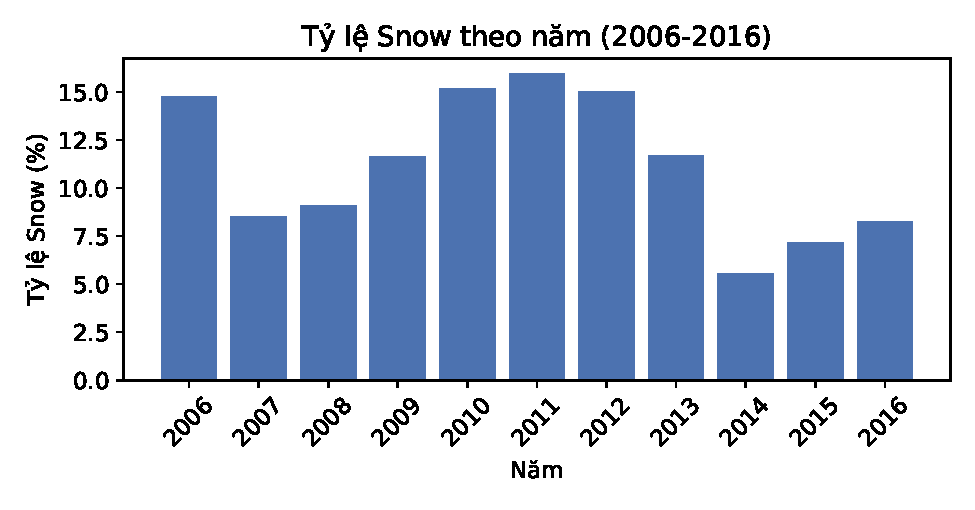
\includegraphics[width=0.78\textwidth]{figs/eda_snow_by_year.pdf}
\caption{Tỷ lệ Snow theo năm, 2006--2016.}
\label{fig:eda-snow-year}
\end{figure}

\begin{figure}[H]
\centering
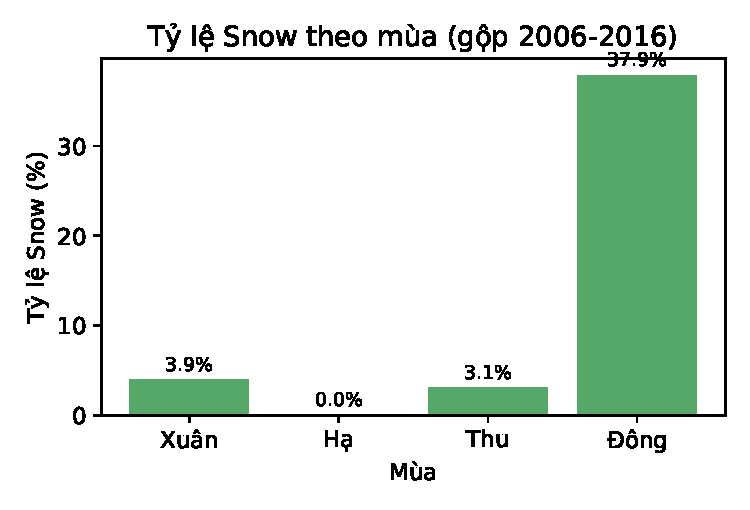
\includegraphics[width=0.62\textwidth]{figs/eda_snow_by_season.pdf}
\caption{Tỷ lệ Snow theo mùa, gộp toàn bộ 2006--2016.}
\label{fig:eda-snow-season}
\end{figure}

\paragraph{Phân bố nhiệt độ theo nhãn.} Hình~\ref{fig:eda-temp-label} vẽ phân bố nhiệt độ
của các bản ghi Rain và Snow. Phát hiện đáng chú ý: trên bộ dữ liệu này, \textbf{nhãn tách
gần như tuyệt đối theo dấu của nhiệt độ} -- toàn bộ 10.712 bản ghi Snow có nhiệt độ
$\le 0$\textdegree C (nhỏ nhất $-21{,}8$\textdegree C, lớn nhất đúng bằng
$0{,}0$\textdegree C), và toàn bộ 85.200 bản ghi Rain có nhiệt độ $> 0$\textdegree C (nhỏ
nhất $0{,}006$\textdegree C). Không tồn tại một bản ghi Rain nào ở nhiệt độ âm, cũng như
không có bản ghi Snow nào ở nhiệt độ dương. Quan sát này củng cố nghi vấn đã nêu ở
Mục~\ref{sec:han-che-nhan}: nhãn \texttt{Precip Type} của Dark Sky API nhiều khả năng cũng
được suy ra (một phần) từ chính ngưỡng nhiệt độ $0$\textdegree C khi có giáng thủy, chứ
không phải một quan trắc loại giáng thủy độc lập với nhiệt độ.

\begin{figure}[H]
\centering
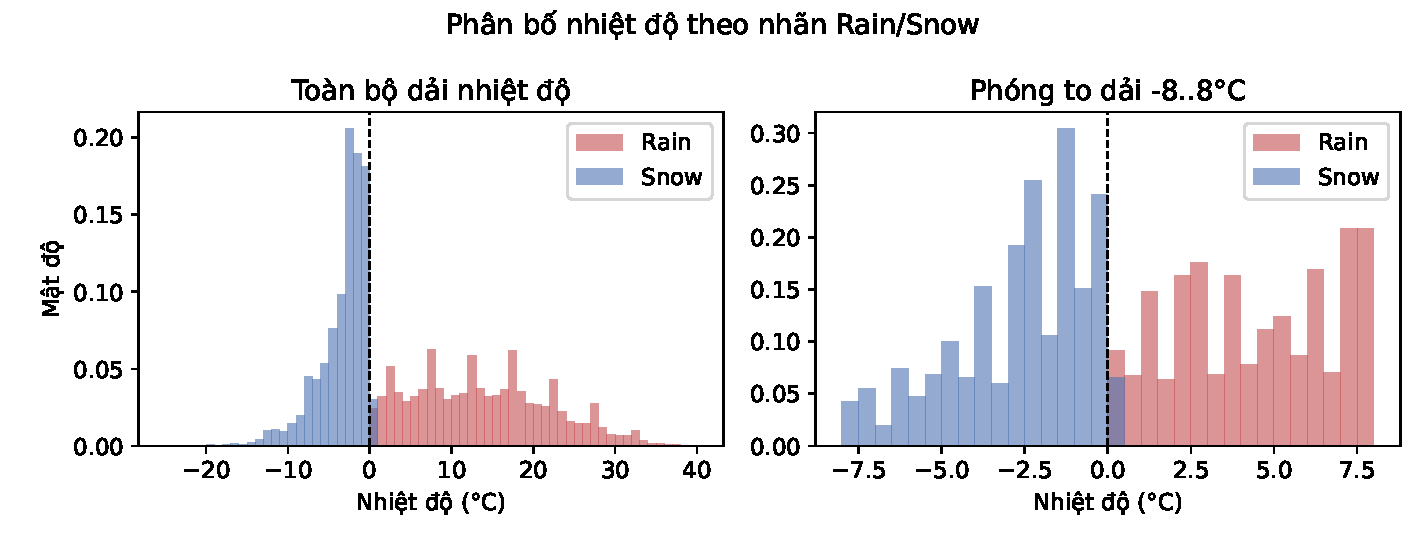
\includegraphics[width=0.95\textwidth]{figs/eda_temperature_by_label.pdf}
\caption{Phân bố nhiệt độ theo nhãn Rain/Snow -- toàn dải (trái) và phóng to quanh
ngưỡng $0$\textdegree C (phải). Đường nét đứt đánh dấu $0$\textdegree C.}
\label{fig:eda-temp-label}
\end{figure}

Vì vậy, cách gọi "\emph{vùng chồng lấn}" cần được hiểu chính xác hơn trên bộ dữ liệu này:
không phải hai lớp có giá trị nhiệt độ trùng nhau, mà là một \emph{dải gần ngưỡng} nơi phần
lớn các trường hợp Snow tập trung sát $0$\textdegree C thay vì rải đều ra các giá trị rất
âm. Cụ thể, trong dải $[-4, 4]$\textdegree C có 19.685 bản ghi, chiếm 38,4\% là Snow -- cao
hơn hẳn tỷ lệ nền 11,2\% -- cho thấy đây là dải nhiệt độ mà việc phân loại nhạy cảm nhất với
sai số hoặc giá trị thiếu của biến nhiệt độ. Nói cách khác: trên dữ liệu \emph{đầy đủ}, một
ngưỡng nhiệt độ đơn giản gần như giải quyết trọn vẹn bài toán (baseline ngưỡng nhiệt độ ở
Mục~\ref{sec:baseline} vì vậy được kỳ vọng rất mạnh khi không thiếu dữ liệu); nhưng khi
nhiệt độ bị thiếu theo kịch bản giả lập ở Mục~\ref{sec:gia-lap-mat-du-lieu} -- đặc biệt với
các bản ghi nằm trong dải sát ngưỡng này -- mô hình buộc phải dựa vào các biến tương quan
khác (độ ẩm, áp suất, gió) hoặc nội suy thay vì chỉ nhìn vào nhiệt độ, và đây chính là phần
việc khó thực sự mà đồ án muốn đánh giá.

\subsection{Hướng xử lý mất cân bằng dữ liệu}
\label{sec:xu-ly-mat-can-bang}

Tỷ lệ Rain:Snow xấp xỉ 8:1 (Mục~\ref{sec:eda}) khiến một mô hình không xử lý gì có thể đạt
Accuracy cao giả tạo (88,8\% chỉ bằng cách luôn đoán Rain) trong khi gần như không nhận ra
được Snow -- đúng là hành vi của baseline lớp đa số (Mục~\ref{sec:baseline}). Đồ án xử lý
vấn đề này ở \textbf{hai tầng độc lập}, áp dụng đồng thời:

\begin{enumerate}
  \item \textbf{Tầng đánh giá (không phụ thuộc thuật toán):} dùng \textbf{Macro F1} và
        \textbf{PR-AUC} làm chỉ số chính thay vì Accuracy (Mục~\ref{sec:metrics}) -- hai chỉ
        số này không bị "pha loãng" bởi lớp đa số, nên vẫn phản ánh đúng chất lượng kể cả
        khi không áp dụng bất kỳ kỹ thuật cân bằng nào ở bước huấn luyện.
  \item \textbf{Tầng thuật toán:} mỗi nhánh/baseline có cơ chế xử lý mất cân bằng riêng,
        phù hợp với bản chất mô hình (Bảng~\ref{tab:xu-ly-mat-can-bang}).
\end{enumerate}

\begin{table}[H]
\centering
\caption{Hướng xử lý mất cân bằng lớp theo từng thành phần.}
\label{tab:xu-ly-mat-can-bang}
\small
\begin{tabular}{@{}p{3.5cm}p{3.1cm}p{7.3cm}@{}}
\toprule
\textbf{Thành phần} & \textbf{Chiến lược} & \textbf{Cơ chế} \\
\midrule
Baseline Logistic Regression & \texttt{class\_weight}\newline\texttt{="balanced"} & Trọng số mỗi lớp tỷ lệ nghịch tần suất, áp trực tiếp vào hàm mất mát (\texttt{evaluation/baselines.py}). \\
\addlinespace
Baseline k-NN & Không xử lý & \texttt{KNeighborsClassifier} của scikit-learn không hỗ trợ trọng số lớp; giữ nguyên làm baseline "thô". \\
\addlinespace
Classic ML (XGBoost) & \texttt{scale\_pos\_weight}\newline (mặc định) hoặc SMOTE & \texttt{scale\_pos\_weight} = (số Rain)/(số Snow) trên tập train; SMOTE sinh thêm mẫu Snow tổng hợp trước khi huấn luyện (\texttt{models/classic.py}, \texttt{trainers/classic\_trainer.py}) -- so sánh hai chiến lược ở Mục~\ref{sec:ablation}. \\
\addlinespace
ROCKET (RidgeClassifierCV) & \texttt{class\_weight}\newline\texttt{="balanced"} & Trọng số nghịch tần suất lớp trong hàm mất mát ridge, đồng nhất với baseline Logistic Regression (\texttt{models/rocket.py}). \\
\addlinespace
Deep Learning\newline (mọi mô hình GRU/BRITS/SAITS) & Cross-entropy\newline có trọng số lớp & Trọng số lớp $c$ = $N / (2 \times \text{số mẫu lớp } c)$, áp cho cả vòng lặp huấn luyện tự cài lẫn \texttt{WeightedCrossEntropy} tuỳ biến cho PyPOTS (\texttt{trainers/deep\_trainer.py}). \\
\bottomrule
\end{tabular}
\end{table}

Baseline persistence và ngưỡng nhiệt độ không cần xử lý mất cân bằng: đây là các quy tắc
đơn giản (tra nhãn quá khứ, so sánh ngưỡng), không học qua một hàm mất mát nên khái niệm
"trọng số lớp" không áp dụng được. Với nhánh Classic ML, cả ba lựa chọn -- không xử lý,
\texttt{scale\_pos\_weight}, SMOTE -- đều được chạy và so sánh trực tiếp bằng Macro F1 ở
Mục~\ref{sec:ablation}, để trả lời câu hỏi kỹ thuật cân bằng nào thực sự cải thiện kết quả
trên bộ dữ liệu này thay vì mặc định chọn một chiến lược.

\subsection{Vấn đề chất lượng dữ liệu}
\label{sec:chat-luong-du-lieu}

Quá trình khảo sát dữ liệu phát hiện bốn vấn đề chất lượng cần xử lý trước khi huấn
luyện, đều được xử lý tự động trong \texttt{datasets/szeged.py:clean()}:

\begin{itemize}
  \item \textbf{Áp suất bằng 0:} \textbf{1.288 dòng} (1,3\% tổng số dòng gốc) có
        \texttt{Pressure~(millibars)~=~0} -- giá trị phi vật lý (áp suất khí quyển không
        thể bằng 0), được xem như giá trị thiếu và chuyển thành NaN.
  \item \textbf{Timestamp trùng:} \textbf{24 dòng} có mốc thời gian trùng với dòng ngay
        trước đó; bản ghi trùng bị loại, chỉ giữ bản ghi xuất hiện đầu tiên.
  \item \textbf{Cột hằng số:} cột \texttt{Loud Cover} chỉ nhận đúng một giá trị (0) trong
        toàn bộ 96.453 dòng, không mang thông tin phân biệt, nên bị loại khỏi tập đặc
        trưng đầu vào.
  \item \textbf{Nhãn bị thiếu:} \textbf{517 dòng} (0,5\%) có \texttt{Precip Type} rỗng
        hoặc khác \texttt{rain}/\texttt{snow}; các dòng này bị loại khỏi tập có nhãn hợp lệ
        nhưng \emph{vẫn được giữ lại} trong lưới giờ liên tục (giá trị đặc trưng của chúng
        vẫn dùng được làm ngữ cảnh lịch sử cho các cửa sổ khác, chỉ riêng nhãn bị đánh dấu
        thiếu) -- xem thêm Mục~\ref{sec:phat-bieu-bai-toan} về cách cửa sổ bị loại nếu nhãn
        tại $t+1$ không hợp lệ.
\end{itemize}

Ngoài ra, sau khi quy dữ liệu về lưới giờ liên tục theo từng giờ, phát hiện thêm
\textbf{520 giờ bị hở hoàn toàn} (không có bản ghi gốc nào, chủ yếu trùng với các dòng vừa
bị loại ở trên) -- đây là phần \emph{thiếu dữ liệu tự nhiên} của bộ dữ liệu, độc lập và được
giữ tách biệt với phần mất dữ liệu \emph{giả lập} dùng để đánh giá độ bền vững của mô hình ở
Mục~\ref{sec:gia-lap-mat-du-lieu}.

\subsection{Quy trình tiền xử lý}
\label{sec:quy-trinh-tien-xu-ly}

Toàn bộ quy trình từ CSV thô đến dữ liệu sẵn sàng huấn luyện gồm bốn bước tự động, lần
lượt nằm trong \texttt{datasets/szeged.py}, \texttt{datasets/windows.py} và
\texttt{datasets/splits.py} (Hình~\ref{fig:pipeline-tien-xu-ly}): \textbf{(1)} đọc và sắp
xếp dữ liệu thô theo thời gian; \textbf{(2)} làm sạch (loại cột hằng số, sửa giá trị phi
vật lý, loại bản ghi trùng/nhãn không hợp lệ, quy về lưới giờ liên tục -- chi tiết ở
Mục~\ref{sec:chat-luong-du-lieu}); \textbf{(3)} cắt cửa sổ trượt 24 giờ, gán nhãn tại giờ
$t{+}1$ ngay sau mỗi cửa sổ; \textbf{(4)} chia tập train/validation/test theo năm.

\begin{figure}[H]
\centering
\resizebox{0.78\textwidth}{!}{%
\begin{tikzpicture}[
  data/.style={rectangle, rounded corners, draw=black, fill=orange!15,
               minimum width=7.2cm, minimum height=1.0cm, align=center, font=\small},
  proc/.style={rectangle, draw=black, fill=blue!15,
               minimum width=7.2cm, minimum height=1.3cm, align=center, font=\small},
  split/.style={rectangle, rounded corners, draw=black, fill=orange!15,
                minimum width=2.2cm, minimum height=1.0cm, align=center, font=\small},
  arr/.style={thick, ->, >=stealth}
]
  \node[data] (csv) {CSV thô\\96.453 dòng $\times$ 12 cột};
  \node[proc, below=0.5cm of csv] (load) {\texttt{load\_raw()}\\Parse timestamp (UTC, naive), sắp xếp theo thời gian};
  \node[proc, below=0.5cm of load] (clean) {\texttt{clean()}\\Loại \texttt{Loud Cover} $\cdot$ Pressure=0$\to$NaN $\cdot$ dedupe\\ $\cdot$ lọc nhãn không hợp lệ $\cdot$ reindex lưới giờ liên tục};
  \node[data, below=0.5cm of clean] (cleaned) {DataFrame sạch: 96.432 dòng (lưới giờ liên tục)\\95.912 dòng có nhãn Rain/Snow hợp lệ};
  \node[proc, below=0.5cm of cleaned, minimum height=1.0cm] (window) {\texttt{build\_windows(window=24)}\\Cửa sổ trượt 24 giờ $\to$ nhãn tại $t{+}1$};
  \node[data, below=0.5cm of window] (windowed) {$X$: (95.888, 24, 5) $\quad$ $y$: (95.888,)};
  \node[proc, below=0.5cm of windowed, minimum height=1.0cm] (split) {\texttt{year\_split()}\\Chia theo năm, chống rò rỉ dữ liệu};
  \node[split, below=0.6cm of split, xshift=-2.6cm] (train) {Train\\69.962};
  \node[split, below=0.6cm of split] (val) {Val\\8.757};
  \node[split, below=0.6cm of split, xshift=2.6cm] (test) {Test\\17.169};

  \draw[arr] (csv) -- (load);
  \draw[arr] (load) -- (clean);
  \draw[arr] (clean) -- (cleaned);
  \draw[arr] (cleaned) -- (window);
  \draw[arr] (window) -- (windowed);
  \draw[arr] (windowed) -- (split);
  \draw[arr] (split) -- (train);
  \draw[arr] (split) -- (val);
  \draw[arr] (split) -- (test);
\end{tikzpicture}}
\caption{Quy trình tiền xử lý: từ CSV thô đến ba tập train/validation/test.}
\label{fig:pipeline-tien-xu-ly}
\end{figure}

Hai bước (3) và (4) chưa được mô tả ở Mục~\ref{sec:chat-luong-du-lieu}:

\begin{itemize}
  \item \textbf{Cắt cửa sổ trượt (\texttt{build\_windows}):} với mỗi vị trí $i$ trên lưới
        giờ liên tục, đặc trưng là 24 giờ $[i-23, i]$, nhãn là giá trị tại giờ $i+1$.
        Cửa sổ bị loại nếu nhãn tại $i+1$ không hợp lệ (NaN); \textbf{đặc trưng vẫn được
        giữ} dù một vài giờ trong cửa sổ trùng với phần thiếu dữ liệu tự nhiên
        (Mục~\ref{sec:chat-luong-du-lieu}) -- đây là lựa chọn có chủ đích, để phần thiếu
        tự nhiên (rất nhỏ, 0,42\% tổng số điểm) không bị trộn lẫn với phần mất dữ liệu
        \emph{giả lập} sẽ thêm vào ở Mục~\ref{sec:gia-lap-mat-du-lieu}.
  \item \textbf{Chia tập (\texttt{year\_split}):} chia theo \emph{thời gian}, không xáo
        trộn ngẫu nhiên -- train gồm các cửa sổ có nhãn thuộc 2006--2013, validation thuộc
        2014, test thuộc 2015--2016 (cố định, không dùng để chọn mô hình/siêu tham số).
        Cách chia này mô phỏng đúng kịch bản dự báo thực tế (dự đoán tương lai từ quá khứ)
        và tránh rò rỉ dữ liệu giữa các tập.
\end{itemize}

\subsection{Dữ liệu sau tiền xử lý}
\label{sec:du-lieu-sau-tien-xu-ly}

Sau bốn bước trên, dữ liệu sẵn sàng cho mọi nhánh phương pháp (Chương~\ref{sec:phuong-phap-de-xuat})
là hai mảng NumPy: $X$ kiểu \texttt{float32}, shape $(95{.}888,\ 24,\ 5)$ -- tương ứng
95.888 cửa sổ, mỗi cửa sổ 24 giờ $\times$ 5 biến (Mục~\ref{sec:nguon-du-lieu}) -- và $y$
kiểu \texttt{int64}, shape $(95{.}888,)$ với $y \in \{0 \text{ (Rain)}, 1 \text{ (Snow)}\}$.
Tỷ lệ Snow trong $y$ là 11,2\%, khớp với tỷ lệ trên toàn bộ dữ liệu có nhãn
(Mục~\ref{sec:eda}) -- việc cắt cửa sổ không làm lệch phân bố lớp. $X$ còn chứa NaN tại
0,42\% số điểm, đúng bằng phần thiếu dữ liệu tự nhiên đã nêu ở
Mục~\ref{sec:chat-luong-du-lieu} (chưa tính phần giả lập thêm ở Chương~\ref{sec:phuong-phap-de-xuat}).
Ba tập được đánh chỉ số (không sao chép dữ liệu) theo Mục~\ref{sec:quy-trinh-tien-xu-ly}:
69.962 cửa sổ train, 8.757 validation, 17.169 test.

Bảng~\ref{tab:vi-du-cua-so} minh hoạ cụ thể một cửa sổ thật (cửa sổ đầu tiên của tập
train): 24 giờ từ 31/12/2005 23:00 đến 01/01/2006 22:00 là đặc trưng đầu vào, nhãn
Rain được lấy từ giờ \textbf{01/01/2006 23:00} -- đúng là giờ ngay sau cửa sổ, không phải
giờ cuối cùng của cửa sổ.

\begin{table}[H]
\centering
\caption{Ví dụ một cửa sổ đầu vào thật (rút gọn, chỉ hiện 3 giờ đầu và 3 giờ cuối trong 24 giờ).}
\label{tab:vi-du-cua-so}
\small
\begin{tabular}{@{}lccccc@{}}
\toprule
Giờ & Temp. (°C) & Humidity & Wind (km/h) & Pressure (mb) & Visib. (km) \\
\midrule
31/12 23:00 & 0,58 & 0,89 & 17,11 & 1016,66 & 9,98 \\
01/01 00:00 & 1,16 & 0,85 & 16,62 & 1016,15 & 9,90 \\
01/01 01:00 & 1,67 & 0,82 & 20,25 & 1015,87 & 9,90 \\
\multicolumn{6}{c}{$\vdots$ (18 giờ còn lại)} \\
01/01 20:00 & 4,93 & 0,86 & 23,94 & 1009,43 & 15,73 \\
01/01 21:00 & 5,47 & 0,87 & 22,72 & 1009,51 & 14,80 \\
01/01 22:00 & 5,42 & 0,86 & 19,56 & 1009,64 & 15,65 \\
\bottomrule
\end{tabular}

\vspace{2pt}
\footnotesize Nhãn tại $t{+}1$ = 01/01 \textbf{23:00} $\to$ \textbf{Rain} ($y=0$).
\end{table}

\subsection{Sinh mặt nạ thiếu dữ liệu giả lập}
\label{sec:sinh-mat-na}

Phần thiếu dữ liệu \emph{tự nhiên} của bộ dữ liệu rất nhỏ (0,42\% số điểm,
Mục~\ref{sec:du-lieu-sau-tien-xu-ly}) -- không đủ để đánh giá mô hình hoạt động tốt đến
đâu khi cảm biến thực sự mất số đo. Vì vậy, ngay trên $X$ đã tiền xử lý, đồ án \textbf{giả
lập thêm} mất dữ liệu theo ba kiểu, ở ba tỷ lệ 10/30/50\% (mô tả đầy đủ về động cơ và thiết
kế ở Mục~\ref{sec:gia-lap-mat-du-lieu}; phần này trình bày cụ thể mặt nạ được sinh ra như
thế nào và trông như thế nào trên dữ liệu thật):

\begin{itemize}
  \item \textbf{Point:} từng điểm $(giờ, biến)$ bị ẩn độc lập, chọn ngẫu nhiên không lặp
        trong số các điểm đang quan sát được -- mô phỏng nhiễu đo/lỗi gói tin rời rạc.
  \item \textbf{Subsequence:} nhiều đoạn liên tiếp ngắn/vừa (độ dài ngẫu nhiên, tối đa nửa
        cửa sổ), mỗi đoạn trên \emph{một} biến -- mô phỏng mất kết nối tạm thời.
  \item \textbf{Block:} một hoặc nhiều biến bị ẩn \emph{toàn bộ} trong một đoạn thời gian
        dài (tối thiểu nửa cửa sổ) -- mô phỏng một cảm biến hỏng hẳn trong thời gian dài.
\end{itemize}

Với mỗi cửa sổ, \texttt{datasets/missingness.py:generate\_mask()} tính trước một
\emph{ngân sách} = (tỷ lệ mục tiêu $\times$ 120 điểm/cửa sổ) $-$ (số điểm đã thiếu tự
nhiên), rồi chọn đúng số điểm đó để ẩn thêm theo kiểu tương ứng -- nhờ vậy tỷ lệ thiếu
\emph{thực tế} luôn sát tỷ lệ mục tiêu dù dữ liệu vốn đã có một ít NaN tự nhiên
(Bảng~\ref{tab:ty-le-mat-du-lieu-thuc-te}). Mặt nạ được sinh với \textbf{seed cố định}
một lần duy nhất và lưu cache (\texttt{outputs/masks/}), để cả ba nhánh phương pháp dùng
chung đúng một mặt nạ cho mỗi cấu hình -- điều kiện bắt buộc để so sánh công bằng.

\begin{figure}[H]
\centering
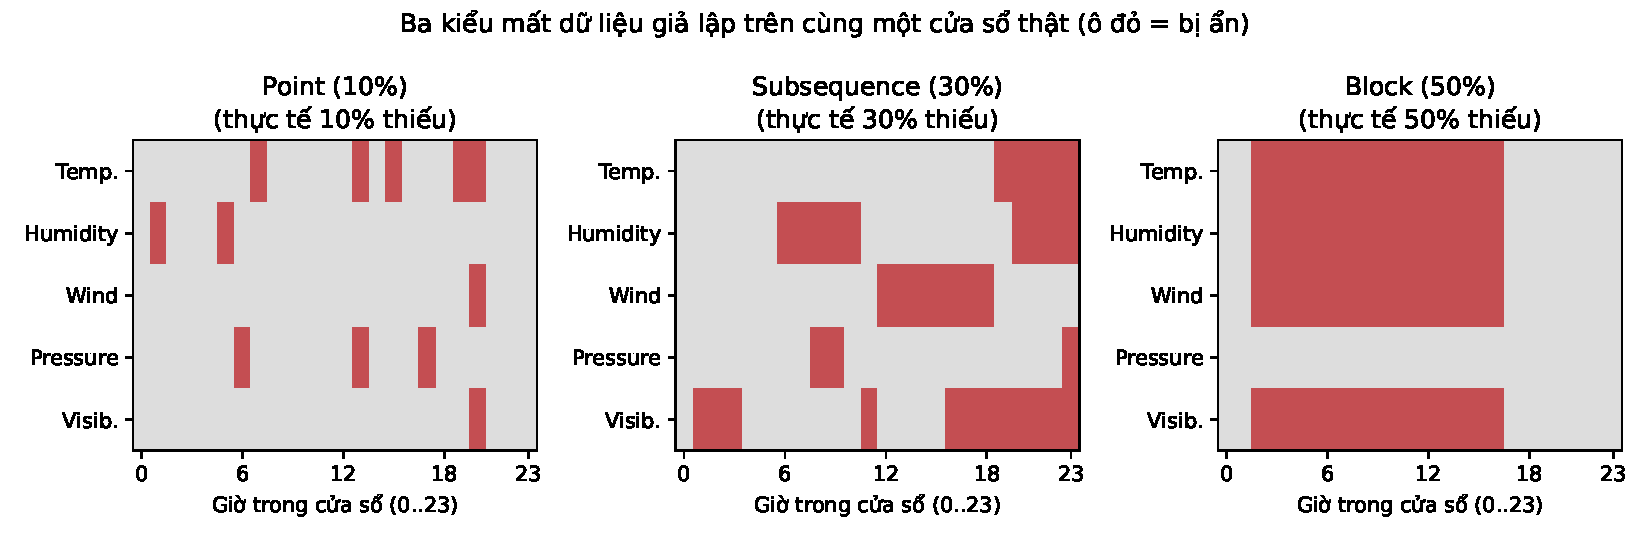
\includegraphics[width=0.95\textwidth]{figs/missingness_mask_example.pdf}
\caption{Ba kiểu mất dữ liệu giả lập áp lên \emph{cùng một} cửa sổ 24 giờ $\times$ 5 biến
thật (không có NaN tự nhiên để mặt nạ hiện rõ): point rải rác từng điểm, subsequence tạo
đoạn liên tiếp trên từng biến, block xoá nguyên biến trong một khoảng thời gian dài.}
\label{fig:missingness-example}
\end{figure}

\begin{table}[H]
\centering
\caption{Tỷ lệ thiếu mục tiêu so với thực tế, đo trên toàn bộ 95.888 cửa sổ (seed=123).}
\label{tab:ty-le-mat-du-lieu-thuc-te}
\small
\begin{tabular}{@{}lccc@{}}
\toprule
\textbf{Kiểu} & \textbf{Mục tiêu 10\%} & \textbf{Mục tiêu 30\%} & \textbf{Mục tiêu 50\%} \\
\midrule
Point & 10,14\% & 30,06\% & 50,02\% \\
Subsequence & 10,14\% & 30,06\% & 50,02\% \\
Block & 10,14\% & 30,06\% & 50,02\% \\
\bottomrule
\end{tabular}
\end{table}

Sai lệch nhỏ và đều giữa ba kiểu (ví dụ 10,14\% thay vì đúng 10,00\%) đến từ việc làm tròn
ngân sách về số nguyên trên từng cửa sổ 120 điểm, cộng thêm 0,42\% đã thiếu sẵn tự nhiên --
không phải do lỗi thuật toán, và sai lệch này giống hệt nhau ở cả ba kiểu vì cùng dùng
chung một công thức ngân sách.

\subsection{Hạn chế của nhãn}
\label{sec:han-che-nhan}

Nhãn Rain/Snow trong bộ dữ liệu Szeged không phải là kết quả quan trắc trực tiếp từ trạm
khí tượng, mà được sinh ra từ dịch vụ Dark Sky API dựa trên mô hình nội suy/dự báo của
bên thứ ba. Phát hiện ở Mục~\ref{sec:eda} -- nhãn tách gần như tuyệt đối theo dấu của
nhiệt độ, không có một ngoại lệ nào trong hơn 95 nghìn bản ghi -- củng cố khả năng nhãn này
\emph{chính nó} đã được suy ra (một phần) từ nhiệt độ bằng một quy tắc tương tự, chứ không
phải một quan trắc loại giáng thủy độc lập. Do đó, mọi so sánh hiệu năng giữa các phương
pháp trong báo cáo này cần được hiểu là so sánh dựa trên nhãn suy ra từ Dark Sky, không
phải nhãn quan trắc thực địa tuyệt đối; một mô hình "học được đúng ngưỡng nhiệt độ" có thể
đơn giản là đang học lại chính quy tắc đã sinh ra nhãn, chứ chưa chắc phản ánh khả năng
phân biệt Rain/Snow trong các tình huống phức tạp hơn (ví dụ mưa đóng băng, mưa tuyết hỗn
hợp) mà quy tắc đơn giản này không có bản ghi nào để phân biệt. Hạn chế này được thảo luận
lại ở Mục~\ref{sec:han-che}.

\newpage
\section{Các Công trình Liên quan}
\label{sec:tong-quan-tai-lieu}

\subsection{Phân loại pha giáng thủy}
\label{sec:lit-phan-loai-giang-thuy}

Hướng tiếp cận truyền thống nhất để phân biệt mưa và tuyết là áp một ngưỡng nhiệt độ
không khí hoặc nhiệt độ ướt (wet-bulb temperature) cố định hoặc theo vùng khí hậu
\cite{jennings2018}. Các nghiên cứu này cho thấy ngưỡng tối ưu thay đổi đáng kể theo vị
trí địa lý và mùa, và luôn tồn tại một dải nhiệt độ chồng lấn mà bản thân nhiệt độ không
đủ để phân biệt hai pha. Các công trình gần đây hơn \cite{webb2025} đặt vấn đề học máy
cho bài toán này, chỉ ra rằng mô hình học máy có thể khai thác thêm thông tin từ độ ẩm,
áp suất và gió để cải thiện độ chính xác trong vùng chồng lấn, nhưng phần lớn các nghiên
cứu này giả định dữ liệu đầu vào đầy đủ.

\textbf{Hệ quả cho đồ án:} ngưỡng nhiệt độ được dùng làm baseline tối thiểu
(Mục~\ref{sec:baseline}), còn các mô hình học máy/học sâu được kỳ vọng vượt baseline này
đặc biệt trong dải nhiệt độ chồng lấn và khi dữ liệu bị thiếu.

\subsection{Trích xuất đặc trưng chuỗi thời gian và mô hình cây}
\label{sec:lit-feature-tree}

Một hướng tiếp cận phổ biến cho phân loại chuỗi thời gian là trích xuất một tập đặc
trưng thống kê/thời gian-tần số từ mỗi cửa sổ, sau đó đưa vào một mô hình phân loại dạng
bảng. Các bộ công cụ tiêu biểu gồm tsfresh \cite{christ2018tsfresh}, trích xuất hàng trăm
đặc trưng tự động có kiểm định ý nghĩa thống kê, và catch22 \cite{lubba2019catch22}, một
tập 22 đặc trưng rút gọn được chọn để vừa có tính phân biệt cao vừa giảm chi phí tính
toán. Kết hợp với các mô hình gradient boosting như XGBoost \cite{chen2016xgboost}, các
phương pháp này thường đạt hiệu năng cạnh tranh với chi phí huấn luyện thấp hơn học sâu.

\textbf{Hệ quả cho đồ án:} nhánh Classic ML (Mục~\ref{sec:nhanh-classic-ml}) kết hợp đặc
trưng catch22/tsfresh với XGBoost, đồng thời khai thác khả năng nhận giá trị thiếu trực
tiếp của XGBoost như một baseline xử lý thiếu dữ liệu đơn giản.

\subsection{Họ ROCKET}
\label{sec:lit-rocket}

Họ ROCKET biến đổi chuỗi thời gian bằng các kernel tích chập và dùng đặc trưng tổng hợp để huấn luyện mô hình tuyến tính. MiniRocket \cite{dempster2021minirocket} sử dụng tập kernel phần lớn xác định, khai thác tỷ lệ phần tử dương (PPV) với các dilation và bias khác nhau. MultiRocket \cite{tan2022multirocket} mở rộng trên chuỗi gốc và sai phân bậc một, sử dụng nhiều phép pooling nhằm làm phong phú biểu diễn đặc trưng.

\textbf{Hệ quả cho đồ án:} cả hai cần đầu vào hữu hạn, nên nhánh ROCKET (Mục~\ref{sec:nhanh-rocket}) nội suy trong cửa sổ lịch sử và nối đặc trưng mask/$\Delta t$ để bổ sung thông tin vị trí thiếu. Thực nghiệm đánh giá các biến thể có ngân sách kernel giảm để phù hợp tài nguyên, không nhằm tái hiện đầy đủ benchmark gốc. Kết quả chỉ được so sánh trong giao thức Szeged của đồ án.

\subsection{RNN xử lý dữ liệu thiếu}
\label{sec:lit-rnn-missing}

GRU-D \cite{che2018grud} mở rộng GRU bằng cách đưa trực tiếp mặt nạ thiếu dữ liệu và thời
gian trôi qua từ lần quan trắc hợp lệ gần nhất ($\Delta t$) vào cổng decay của trạng thái
ẩn và của giá trị đầu vào, cho phép mô hình "quên" có kiểm soát khi dữ liệu thiếu kéo
dài. BRITS \cite{cao2018brits} đi theo hướng khác: xây dựng một mô hình imputation hai
chiều (forward/backward) dựa trên RNN, huấn luyện đồng thời với tác vụ phân loại để lan
truyền thông tin ngữ cảnh qua các đoạn thiếu.

\textbf{Hệ quả cho đồ án:} cả hai kiến trúc được triển khai trong nhánh Deep Learning
(Mục~\ref{sec:nhanh-deep-learning}) cùng với một mô hình GRU đơn giản có mask/$\Delta t$
làm đặc trưng bổ sung (GRU-Fill), nhằm đo đóng góp riêng của cơ chế decay có kiểm soát.

\subsection{Transformer và mô hình nền tảng}
\label{sec:lit-transformer}

SAITS \cite{du2023saits} dùng cơ chế self-attention với một mục tiêu kép (joint-optimization
giữa imputation và dự đoán) để tránh phải xây hai pha huấn luyện riêng biệt như BRITS.
Các mô hình nền tảng chuỗi thời gian đa nhiệm gần đây, ví dụ UniTS \cite{gao2024units},
được huấn luyện trước trên nhiều bộ dữ liệu và nhiều tác vụ (dự báo, phân loại,
imputation), cho phép fine-tune trên một bài toán cụ thể với lượng dữ liệu huấn luyện ít
hơn.

\textbf{Hệ quả cho đồ án:} SAITS được đưa vào như đại diện cho hướng attention-based
imputation, và UniTS (nếu đủ thời gian/tài nguyên) được dùng để kiểm tra liệu fine-tuning
từ một mô hình nền tảng có mang lại lợi thế so với huấn luyện từ đầu trên riêng dữ liệu
Szeged.

\subsection{Đánh giá trên Szeged và các benchmark liên quan}
\label{sec:lit-benchmark-szeged}

\TODO{Rà soát các báo cáo/đồ án/kernel công khai đã dùng bộ dữ liệu Szeged (chủ yếu cho
hồi quy nhiệt độ hoặc phân loại Rain/Snow ở điều kiện dữ liệu đầy đủ), và nêu rõ điểm
khác biệt: các công trình này không giả lập hoặc đánh giá dưới điều kiện mất dữ liệu.}

\subsection{Bảng tổng hợp và khoảng trống nghiên cứu}
\label{sec:lit-tong-hop}

\begin{table}[H]
\centering
\caption{Tổng hợp các hướng tiếp cận liên quan và vị trí của đồ án.}
\label{tab:lit-summary}
\begin{tabular}{@{}p{3.1cm}p{4.3cm}p{4.3cm}@{}}
\toprule
\textbf{Hướng tiếp cận} & \textbf{Giả định chính} & \textbf{Khoảng trống so với đồ án} \\
\midrule
Ngưỡng nhiệt độ \cite{jennings2018,webb2025} & Dữ liệu đầy đủ, mối quan hệ nhiệt độ--pha giáng thủy ổn định & Không xử lý dữ liệu thiếu; độ chính xác thấp trong vùng chồng lấn \\
Đặc trưng + cây quyết định \cite{christ2018tsfresh,lubba2019catch22,chen2016xgboost} & Cửa sổ đầu vào đầy đủ hoặc thiếu ngẫu nhiên nhẹ & Thiếu đánh giá hệ thống theo nhiều tỷ lệ/kiểu thiếu \\
ROCKET \cite{dempster2021minirocket,tan2022multirocket} & Chuỗi đầu vào liên tục, không thiếu & Cần bước nội suy riêng; chưa có benchmark dưới điều kiện thiếu \\
RNN cho dữ liệu thiếu \cite{che2018grud,cao2018brits} & Thiếu dữ liệu là điều kiện vận hành bình thường & Ít được so sánh trực tiếp với ROCKET/đặc trưng cổ điển trên cùng bài toán \\
Attention/mô hình nền tảng \cite{du2023saits,gao2024units} & Có đủ dữ liệu/tài nguyên để huấn luyện hoặc fine-tune & Chi phí tính toán cao, chưa rõ có cần thiết cho bài toán quy mô một trạm \\
\bottomrule
\end{tabular}
\end{table}

Khoảng trống chung là: chưa có nghiên cứu so sánh trực tiếp ba hướng tiếp cận trên cùng
một bộ dữ liệu, cùng một giao thức giả lập thiếu dữ liệu và cùng một tập chỉ số đánh giá
-- đây chính là mục tiêu của đồ án.

\newpage
\section{Phương pháp đề xuất}
\label{sec:phuong-phap-de-xuat}

\subsection{Tổng quan pipeline}
\label{sec:tong-quan-pipeline}

Hình~\ref{fig:pipeline-overview} minh họa pipeline chung: dữ liệu thô Szeged được làm
sạch và cắt cửa sổ trượt, sau đó một bộ mặt nạ thiếu dữ liệu dùng chung được áp lên cùng
một tập cửa sổ để tạo ra các bản sao bị thiếu ở nhiều tỷ lệ/kiểu khác nhau. Từ đây,
pipeline rẽ thành ba nhánh xử lý độc lập -- Classic ML, ROCKET, và Deep Learning -- mỗi
nhánh có bước tiền xử lý riêng phù hợp với giả định đầu vào của mình, trước khi hội tụ
vào một khâu đánh giá chung (Chương~\ref{sec:thiet-lap-thuc-nghiem}).

\begin{figure}[H]
\centering
\TODO{Vẽ sơ đồ pipeline: Dữ liệu thô → Làm sạch + cắt cửa sổ → Mặt nạ thiếu dữ liệu dùng
chung → rẽ 3 nhánh (Classic ML / ROCKET / Deep Learning) → Đánh giá chung (metrics,
kiểm định thống kê, giải thích mô hình).}
\caption{Tổng quan pipeline của đồ án.}
\label{fig:pipeline-overview}
\end{figure}

Tiền xử lý chung (làm sạch, cắt cửa sổ trượt, chia theo năm, chống rò rỉ dữ liệu) và cách
giả lập mặt nạ thiếu dữ liệu (point/subsequence/block, dùng chung cho mọi nhánh) đã được
trình bày chi tiết ở Mục~\ref{sec:quy-trinh-tien-xu-ly}--\ref{sec:sinh-mat-na}; các mục
dưới đây tập trung vào phần riêng của từng nhánh phương pháp.

\subsection{Nhánh Classic ML}
\label{sec:nhanh-classic-ml}

\subsubsection{Feature engineering}
\label{sec:feature-engineering}

\begin{itemize}
  \item \textbf{LiteStatTemp:} \TODO{định nghĩa chính xác tập đặc trưng thống kê/nhiệt độ
        rút gọn tự thiết kế -- ví dụ mean/std/min/max/slope của từng biến trong cửa sổ,
        cùng một số đặc trưng riêng cho nhiệt độ (ví dụ số lần cắt ngưỡng 0\textdegree C).}
  \item \textbf{Đặc trưng mask/$\Delta t$:} tỷ lệ giá trị thiếu theo biến, độ dài đoạn
        thiếu dài nhất, và thời gian trôi qua từ lần quan trắc hợp lệ gần nhất, được tính
        trực tiếp từ mặt nạ $M$ ở Mục~\ref{sec:sinh-mat-na}.
  \item \textbf{catch22} \cite{lubba2019catch22} và \textbf{tsfresh} \cite{christ2018tsfresh}:
        bộ đặc trưng chuẩn hóa được trích xuất bằng thư viện tương ứng, dùng làm đối
        chứng/mở rộng cho LiteStatTemp.
\end{itemize}

\subsubsection{Xử lý dữ liệu thiếu}
\label{sec:xu-ly-thieu-classic-ml}

Ba cách xử lý dữ liệu thiếu được so sánh ở nhánh này:

\begin{enumerate}
  \item \textbf{XGBoost nhận NaN trực tiếp} \cite{chen2016xgboost}: khai thác khả năng
        học hướng phân nhánh tối ưu cho giá trị thiếu ngay trong quá trình huấn luyện
        cây, không cần bước impute riêng.
  \item \textbf{Median kèm mask:} điền giá trị thiếu bằng trung vị (ước lượng trên tập
        huấn luyện) và bổ sung đặc trưng mask tương ứng, làm baseline impute đơn giản.
  \item \textbf{MissForest} \cite{stekhoven2012missforest}: impute lặp dựa trên random
        forest, khai thác tương quan giữa các biến để ước lượng giá trị thiếu tốt hơn
        median.
\end{enumerate}

\subsubsection{Xử lý mất cân bằng lớp}
\label{sec:mat-can-bang-lop-classic}

\TODO{Xác nhận mức độ mất cân bằng Rain/Snow thực tế (xem Mục~\ref{sec:eda}) và chọn
chiến lược xử lý -- ví dụ \texttt{scale\_pos\_weight} của XGBoost, hoặc oversampling
(SMOTE) trên tập huấn luyện -- so sánh các chiến lược này ở Mục~\ref{sec:ablation}.}

\subsubsection{Hyperparameter tuning}
\label{sec:tuning-classic-ml}

Siêu tham số của XGBoost (độ sâu cây, learning rate, số lượng cây, subsample,
colsample\_bytree, min\_child\_weight) được tối ưu bằng Optuna \cite{akiba2019optuna},
với hàm mục tiêu là Macro F1 trung bình trên các fold validation (Mục~\ref{sec:giao-thuc-chia-du-lieu}).
\TODO{Ghi lại không gian tìm kiếm cụ thể cho từng siêu tham số và số lượng trial đã
chạy.}

\subsection{Nhánh ROCKET}
\label{sec:nhanh-rocket}

MiniRocket \cite{dempster2021minirocket} và MultiRocket \cite{tan2022multirocket} yêu cầu
đầu vào không có giá trị thiếu, do đó mỗi cửa sổ bị thiếu được nội suy tuyến tính theo
thời gian cho từng biến trước khi đưa vào bộ biến đổi kernel ngẫu nhiên; các đoạn thiếu ở
đầu/cuối cửa sổ được điền bằng giá trị hợp lệ gần nhất (forward/backward fill). Đặc trưng
đầu ra của MiniRocket/MultiRocket sau đó được đưa vào một mô hình tuyến tính (ridge
classifier) để phân loại. Việc nội suy trước khi biến đổi khiến nhánh này "mù" với vị trí
thiếu gốc trừ khi đặc trưng mask/$\Delta t$ ở Mục~\ref{sec:feature-engineering} được nối
thêm vào đặc trưng ROCKET trước khi phân loại.

\subsection{Nhánh Deep Learning}
\label{sec:nhanh-deep-learning}

\subsubsection{Tiền xử lý riêng cho Deep Learning}
\label{sec:tien-xu-ly-dl}

Mỗi biến được chuẩn hóa (z-score, thống kê ước lượng trên tập huấn luyện), và với mỗi
cửa sổ, hai kênh phụ được tạo thêm cho mỗi biến: kênh \emph{mask} (1 nếu quan trắc hợp
lệ, 0 nếu thiếu) và kênh \emph{delta} ($\Delta t$, thời gian trôi qua từ lần quan trắc
hợp lệ gần nhất của biến đó). Đầu vào mô hình do đó có 3 kênh cho mỗi biến gốc (giá trị,
mask, delta).

\paragraph{Đầu vào riêng của SAITS trong thực nghiệm đã chạy.}
SAITS nhận tensor giá trị có kích thước $(B,24,5)$, với $B$ là batch size và các
ô thiếu vẫn mang giá trị NaN tại giao diện \texttt{fit}/\texttt{predict}. Năm biến
theo thứ tự là nhiệt độ, độ ẩm, tốc độ gió, áp suất và khả năng nhìn. Lần chạy được
báo cáo đặt \texttt{NORMALIZE=False}, giữ đơn vị gốc của các biến và không bổ sung
kênh $\Delta t$. Dataset bên trong PyPOTS tạo mask $M$ (1: quan sát, 0: thiếu),
thay NaN bằng 0 để tính toán và ghép giá trị với mask trước lớp embedding của SAITS.

\subsubsection{Mô hình}
\label{sec:mo-hinh-dl}

\begin{itemize}
  \item \textbf{GRU-Fill:} GRU chuẩn trên dữ liệu đã được điền giá trị đơn giản (forward
        fill), dùng làm baseline học sâu không khai thác mask/delta.
  \item \textbf{GRU kèm mask và delta:} GRU-Fill mở rộng bằng cách nối thêm kênh mask và
        delta vào đầu vào, không thay đổi kiến trúc cell.
  \item \textbf{GRU-D} \cite{che2018grud}: cổng decay nhận trực tiếp mask và delta để
        điều chỉnh suy giảm ảnh hưởng của giá trị quan trắc cũ.
  \item \textbf{BRITS} \cite{cao2018brits}: imputation hai chiều dựa trên RNN, huấn
        luyện đa mục tiêu (imputation + phân loại).
  \item \textbf{SAITS} \cite{du2023saits}: biến thể phân loại trong PyPOTS, sử dụng
        hai khối DMSA và một head phân loại Rain/Snow, huấn luyện bằng cross-entropy
        có trọng số lớp. Cấu hình thực tế được trình bày tại
        Mục~\ref{sec:saits-cau-hinh-da-chay}.
  \item \textbf{UniTS} \cite{gao2024units} (nếu đủ thời gian/tài nguyên): fine-tune từ
        checkpoint pretrained cho tác vụ phân loại trên dữ liệu Szeged.
\end{itemize}

\subsubsection{Kỹ thuật huấn luyện}
\label{sec:ky-thuat-huan-luyen-dl}

\begin{itemize}
  \item \textbf{Loss có trọng số lớp:} cross-entropy với trọng số tỷ lệ nghịch với tần
        suất lớp, để giảm thiên lệch do mất cân bằng Rain/Snow.
  \item \textbf{Early stopping:} dừng huấn luyện khi Macro F1 trên tập validation không
        cải thiện sau $k$ epoch liên tiếp (\TODO{xác định $k$ cụ thể}).
  \item \textbf{Scheduler:} giảm learning rate theo kế hoạch (\TODO{xác định loại
        scheduler -- cosine annealing hoặc reduce-on-plateau -- và tham số cụ thể}).
  \item \textbf{Nhiều seed:} mỗi mô hình được huấn luyện lại với \TODO{số lượng} seed
        khác nhau để báo cáo trung bình và độ lệch chuẩn của mỗi chỉ số.
\end{itemize}

\subsubsection{Cấu hình SAITS đã sử dụng trong thực nghiệm}
\label{sec:saits-cau-hinh-da-chay}

Mô hình \texttt{pypots.classification.SAITS} được khởi tạo mới cho mỗi cặp điều
kiện thiếu dữ liệu--seed. Mỗi khối DMSA chứa hai encoder layer và bốn attention
head; phép chiếu đầu vào chuyển vector ghép giá trị--mask từ 10 chiều sang
64 chiều, có positional encoding. Hai khối tạo các ước lượng được kết hợp bằng
trọng số học từ mask và attention. Ước lượng kết hợp $(B,24,5)$ được trải phẳng
thành $(B,120)$, qua lớp tuyến tính $120\to2$ và softmax để dự đoán Rain/Snow
tại giờ kế tiếp. Đầu ra điền thiếu của PyPOTS là một nhánh phụ; kết quả thực nghiệm
ở Chương~\ref{sec:ket-qua-va-phan-tich} đánh giá tác vụ phân loại.

\begin{table}[H]
\centering
\caption{Cấu hình SAITS của 30 lượt chạy được báo cáo; đây là cấu hình đã sử dụng,
không phải kết quả tìm kiếm siêu tham số.}
\label{tab:saits-cau-hinh}
\begin{tabular}{@{}p{5.2cm}p{9.8cm}@{}}
\toprule
\textbf{Thành phần} & \textbf{Thiết lập} \\
\midrule
Đầu vào và đầu ra & Cửa sổ $24\times5$; Rain $=0$, Snow $=1$ tại $t+1$ \\
Backbone & Hai khối DMSA; 2 encoder layer mỗi khối; 4 head \\
Kích thước biểu diễn & $d_{\mathrm{model}}=64$, $d_k=d_v=16$, $d_{\mathrm{ffn}}=128$ \\
Regularization & Dropout $=0.1$; attention dropout $=0.1$; bật diagonal attention mask \\
Optimizer & Adam, learning rate cố định $10^{-3}$, không dùng scheduler \\
Huấn luyện & Batch size 128; tối đa 50 epoch; patience 10 \\
Loss và chọn checkpoint & Weighted cross-entropy trên train; chọn validation loss thấp nhất \\
Seed & Mask: 123; huấn luyện: 42, 1, 2 \\
\bottomrule
\end{tabular}
\end{table}

Trọng số lớp được tính trên tập train theo $w_c=N_{\mathrm{train}}/(2N_c)$,
xấp xỉ $0.5729$ cho Rain và $3.9278$ cho Snow. Riêng SAITS sử dụng weighted
cross-entropy trên validation để early stopping và chọn checkpoint, thay cho
tiêu chí Macro F1 nêu trong khung huấn luyện chung ở trên. Sau huấn luyện, mô
hình khôi phục checkpoint tốt nhất rồi dự đoán validation/test bằng argmax
của hai xác suất lớp. Test không tham gia chọn epoch hoặc siêu tham số.

\subsubsection{Fine-tuning}
\label{sec:fine-tuning}

\TODO{Nếu sử dụng UniTS: mô tả checkpoint pretrained được dùng, chiến lược fine-tuning
(toàn phần hoặc chỉ fine-tune head phân loại), và số epoch/learning rate fine-tuning.}

\subsection{Giải thích mô hình}
\label{sec:giai-thich-mo-hinh}

Đóng góp của từng đặc trưng đến quyết định phân loại được phân tích bằng SHAP
\cite{lundberg2017shap} cho các mô hình dạng cây (XGBoost), và bằng Integrated Gradients
\cite{sundararajan2017integratedgradients} cho các mô hình học sâu, nhằm kiểm tra xem các
mô hình có thực sự khai thác thông tin mask/$\Delta t$ khi dữ liệu bị thiếu hay không.
Kết quả giải thích mô hình được trình bày ở Mục~\ref{sec:giai-thich-mo-hinh-ket-qua}.

\newpage
\section{Thiết lập thực nghiệm}
\label{sec:thiet-lap-thuc-nghiem}

\subsection{Giao thức chia dữ liệu}
\label{sec:giao-thuc-chia-du-lieu}

Dữ liệu được chia theo thời gian để mô phỏng kịch bản dự báo thực tế, tránh rò rỉ thông
tin tương lai vào quá trình chọn mô hình: \TODO{xác định cụ thể các fold rolling-origin
dùng cho validation (ví dụ huấn luyện tăng dần theo năm, validate trên năm kế tiếp) và
xác nhận tập test cuối cùng, cố định, là giai đoạn 2015--2016, không được dùng cho bất kỳ
quyết định chọn mô hình hay siêu tham số nào.}

\subsection{Baseline}
\label{sec:baseline}

\begin{itemize}
  \item \textbf{Lớp đa số:} luôn dự đoán lớp xuất hiện nhiều hơn trong tập huấn luyện.
  \item \textbf{Persistence:} dự đoán nhãn tại $t+1$ bằng nhãn quan trắc gần nhất hợp lệ
        trong cửa sổ.
  \item \textbf{Ngưỡng nhiệt độ:} phân loại Snow nếu nhiệt độ dưới một ngưỡng cố định
        (\TODO{xác định ngưỡng, ví dụ hiệu chỉnh trên tập huấn luyện}), tương ứng với
        hướng tiếp cận truyền thống ở Mục~\ref{sec:lit-phan-loai-giang-thuy}.
  \item \textbf{Logistic Regression} và \textbf{k-NN:} trên đặc trưng LiteStatTemp sau
        khi impute bằng median, làm baseline học máy đơn giản không chuyên biệt cho dữ
        liệu thiếu.
\end{itemize}

\subsection{Metrics}
\label{sec:metrics}

\TODO{Lấy định nghĩa và lý do chọn từng chỉ số từ tài liệu metrics của nhóm (ví dụ vì sao
chọn Macro F1 thay vì Accuracy do mất cân bằng lớp, và vì sao bổ sung PR-AUC để đánh giá
độ nhạy với ngưỡng quyết định). Liệt kê đầy đủ: Macro F1, Precision/Recall theo lớp,
PR-AUC, và bất kỳ chỉ số phụ nào khác (ví dụ Balanced Accuracy, Cohen's Kappa).}

\subsection{Kiểm định thống kê}
\label{sec:kiem-dinh-thong-ke}

Sự khác biệt hiệu năng giữa từng cặp mô hình trên cùng tập test được kiểm định bằng
McNemar's test \cite{mcnemar1947}, phù hợp để so sánh hai bộ phân loại trên cùng một tập
dữ liệu. Để so sánh đồng thời nhiều mô hình trên nhiều cấu hình thiếu dữ liệu, kiểm định
Friedman kèm biểu đồ critical difference (CD) \cite{demsar2006statistical} được dùng để
xếp hạng và xác định nhóm mô hình không khác biệt có ý nghĩa thống kê.

\subsection{Môi trường chạy}
\label{sec:moi-truong-chay}

\TODO{Ghi lại phần cứng (CPU/GPU, RAM), phiên bản Python và các thư viện chính (XGBoost,
sktime/aeon cho MiniRocket/MultiRocket, PyTorch cho GRU-D/BRITS/SAITS/UniTS, Optuna), và
danh sách seed cố định dùng cho khả năng tái lập kết quả.}

\newpage
\section{Kết quả và phân tích}
\label{sec:ket-qua-va-phan-tich}

\subsection{Kết quả trên dữ liệu đầy đủ (0\% thiếu)}
\label{sec:ket-qua-du-lieu-day-du}

\begin{table}[H]
\centering
\caption{Hiệu năng của tất cả mô hình và baseline trên tập test, không giả lập thiếu dữ
liệu (0\%).}
\label{tab:ket-qua-day-du}
\begin{tabular}{@{}lcccc@{}}
\toprule
\textbf{Mô hình} & \textbf{Macro F1} & \textbf{PR-AUC} & \textbf{Precision} & \textbf{Recall} \\
\midrule
Lớp đa số & \TODO{} & \TODO{} & \TODO{} & \TODO{} \\
Persistence & \TODO{} & \TODO{} & \TODO{} & \TODO{} \\
Ngưỡng nhiệt độ & \TODO{} & \TODO{} & \TODO{} & \TODO{} \\
Logistic Regression & \TODO{} & \TODO{} & \TODO{} & \TODO{} \\
k-NN & \TODO{} & \TODO{} & \TODO{} & \TODO{} \\
XGBoost (LiteStatTemp) & \TODO{} & \TODO{} & \TODO{} & \TODO{} \\
MiniRocket & \TODO{} & \TODO{} & \TODO{} & \TODO{} \\
MultiRocket & \TODO{} & \TODO{} & \TODO{} & \TODO{} \\
GRU-D & \TODO{} & \TODO{} & \TODO{} & \TODO{} \\
BRITS & \TODO{} & \TODO{} & \TODO{} & \TODO{} \\
SAITS & $0.9224 \pm 0.0082$ & \TODO{} & \TODO{} & \TODO{} \\
\bottomrule
\end{tabular}
\end{table}

\subsection{Kết quả chính: suy giảm hiệu năng theo tỷ lệ thiếu dữ liệu}
\label{sec:ket-qua-chinh}

\subsubsection{Kết quả SAITS đã được đối soát}
\label{sec:saits-ket-qua}

Bảng~\ref{tab:saits-macro-f1-missingness} tổng hợp Macro F1 trên test của SAITS
từ 30 lượt chạy thuộc thí nghiệm \texttt{experiment\_a2a9e03b4630}. Mỗi điều
kiện có đủ ba seed 1, 2 và 42. Kết quả được lấy từ bản đối soát đã kiểm tra lại
dự đoán từng lượt, không lấy từ bảng minh họa hay lượt chạy thử. Dòng SAITS ở
Bảng~\ref{tab:ket-qua-day-du} dùng cùng cách tổng hợp mean $\pm$ sample std.

\begin{table}[H]
\centering
\caption{Macro F1 của SAITS trên test theo điều kiện thiếu dữ liệu. Mean $\pm$
sample std được tính giữa ba seed; chênh lệch là hiệu hai giá trị trung bình,
lấy điều kiện không ẩn thêm làm mốc.}
\label{tab:saits-macro-f1-missingness}
\begin{tabular}{@{}lcc@{}}
\toprule
\textbf{Điều kiện} & \textbf{Macro F1} & \textbf{Chênh lệch so với mốc} \\
\midrule
% Generated from report/data/saits_verified_results.json; SAITS only.
Không ẩn thêm & $0.9224 \pm 0.0082$ & $0.0000$ \\
Point 10\% & $0.9266 \pm 0.0038$ & $+0.0042$ \\
Point 30\% & $0.8200 \pm 0.0154$ & $-0.1024$ \\
Point 50\% & $0.8530 \pm 0.0071$ & $-0.0694$ \\
Subsequence 10\% & $0.9068 \pm 0.0053$ & $-0.0156$ \\
Subsequence 30\% & $0.8681 \pm 0.0062$ & $-0.0543$ \\
Subsequence 50\% & $0.8030 \pm 0.0614$ & $-0.1194$ \\
Block 10\% & $0.9174 \pm 0.0077$ & $-0.0050$ \\
Block 30\% & $0.9085 \pm 0.0084$ & $-0.0139$ \\
Block 50\% & $0.8943 \pm 0.0061$ & $-0.0281$ \\
\bottomrule

\end{tabular}
\end{table}

\begin{figure}[H]
\centering
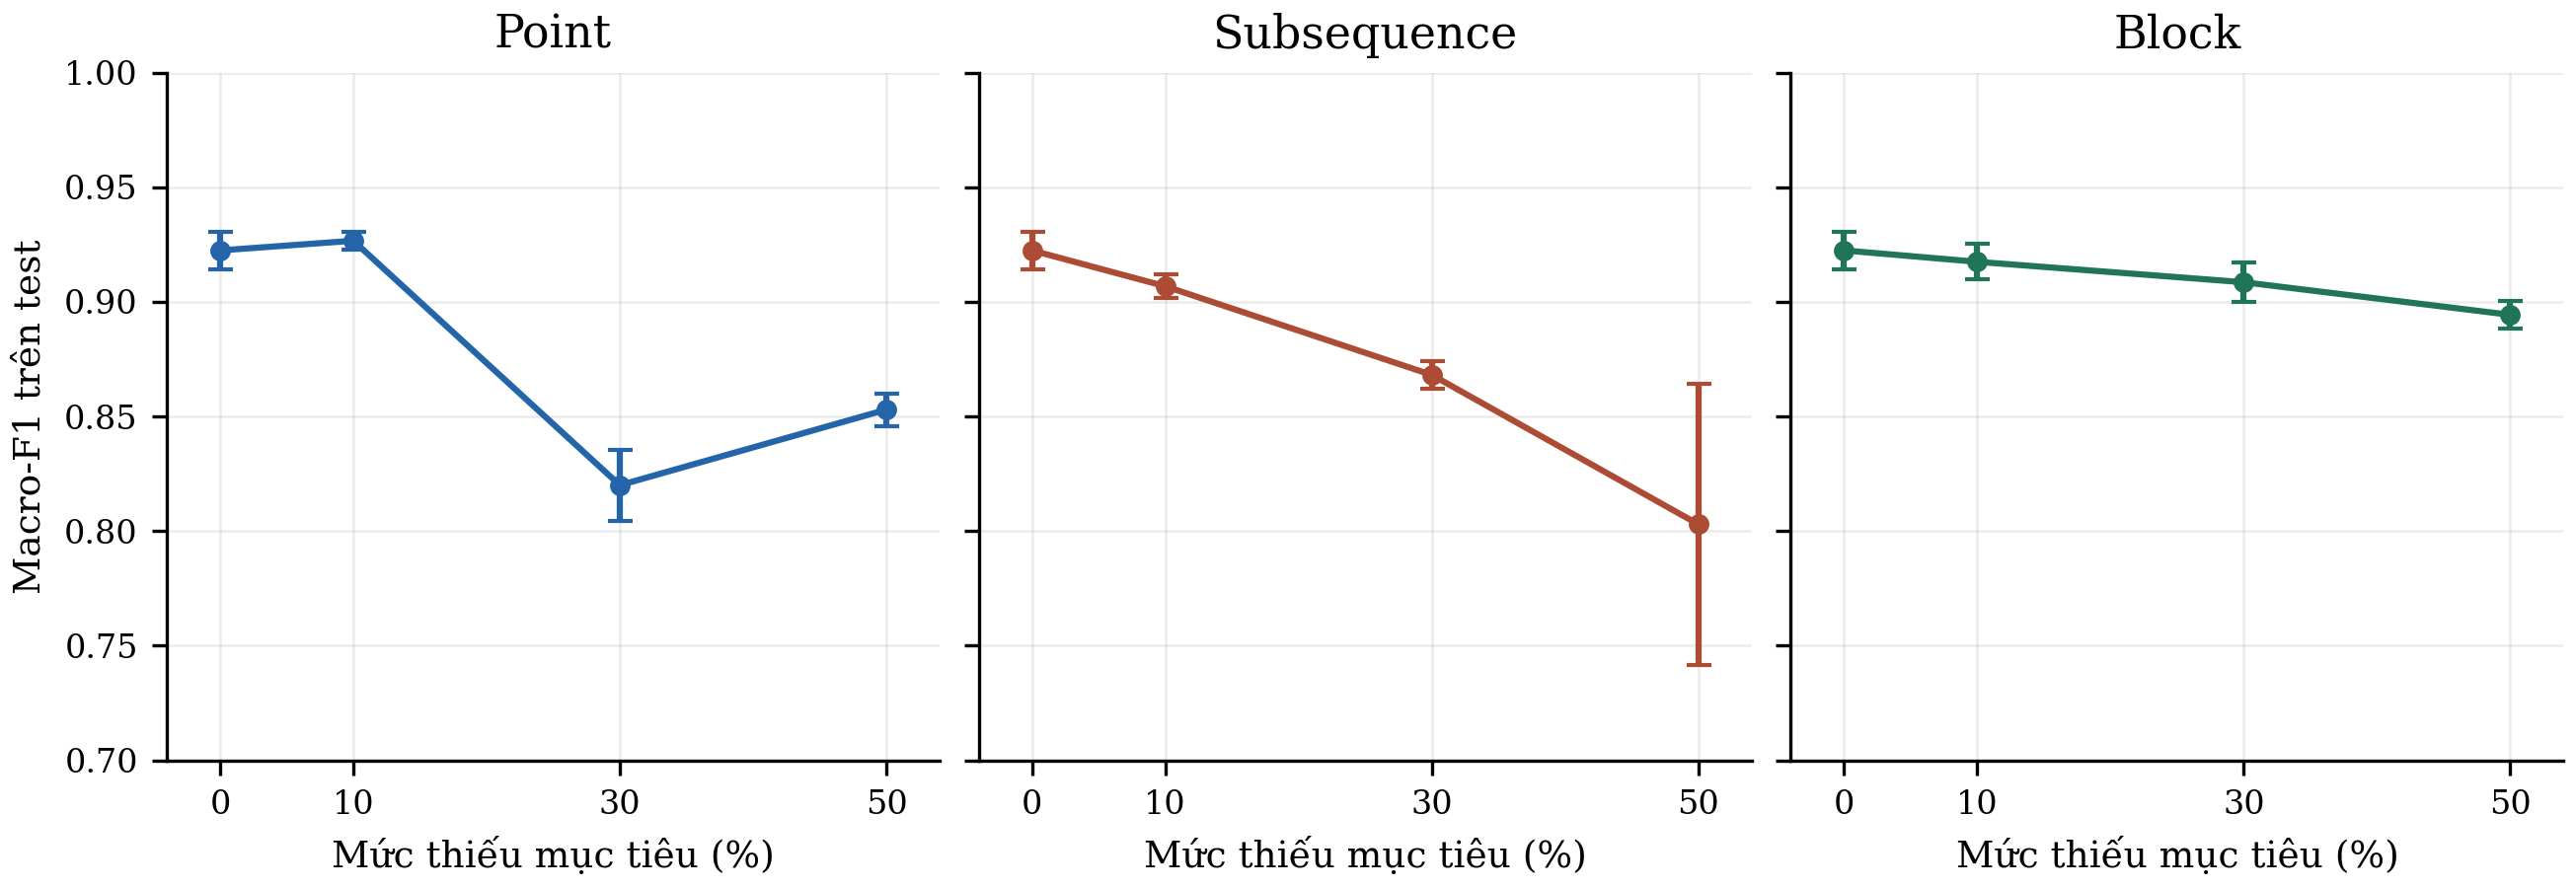
\includegraphics[width=\textwidth]{figs/saits_macro_f1_missingness.png}
\caption{Macro F1 của SAITS theo kiểu và mức thiếu. Điểm là trung bình, thanh
sai số là độ lệch chuẩn mẫu giữa ba seed. Mốc 0\% dùng chung kết quả không ẩn
thêm và vẫn giữ thiếu tự nhiên. Các đường nối chỉ hỗ trợ quan sát xu hướng.}
\label{fig:saits-macro-f1-missingness}
\end{figure}

\paragraph{Ảnh hưởng của mức và kiểu thiếu.}
Không ẩn thêm cho Macro F1 $0.9224 \pm 0.0082$. Ở mức thiếu 50\%, point,
subsequence và block lần lượt đạt $0.8530 \pm 0.0071$, $0.8030 \pm 0.0614$
và $0.8943 \pm 0.0061$, tương ứng giảm khoảng 6.94, 11.94 và 2.81 điểm phần
trăm Macro F1 so với mốc. Trong lần chạy này, block ở mức 30\% và 50\% cho
điểm trung bình cao hơn point/subsequence cùng mức; do đó kết quả SAITS không
ủng hộ nhận định rằng block luôn là kiểu thiếu gây suy giảm mạnh nhất.

\paragraph{Xu hướng không đơn điệu và độ biến thiên giữa seed.}
Point 10\% đạt $0.9266$, nhỉnh hơn mốc không ẩn thêm $0.0042$; point 30\%
đạt $0.8200$, thấp hơn point 50\% ($0.8530$). Vì từng điều kiện được huấn
luyện độc lập, các quan sát này cần được báo cáo nguyên trạng; chưa đủ cơ sở
để kết luận rằng tăng mức thiếu cải thiện mô hình. Subsequence 50\% có độ lệch
chuẩn lớn nhất ($0.0614$): Macro F1 của seed 1, 2 và 42 lần lượt là $0.8411$,
$0.8357$ và $0.7321$ (Phụ lục~\ref{sec:phu-luc-saits-seed}). Sự phân tán này
cho thấy việc báo cáo cả ba seed cần thiết hơn việc chỉ chọn lượt tốt nhất.

\begin{figure}[H]
\centering
\TODO{Vẽ đường suy giảm Macro F1 (và PR-AUC) theo tỷ lệ thiếu dữ liệu (0/10/30/50\%),
mỗi đường ứng với một mô hình, tách thành 3 subplot riêng cho từng kiểu mất dữ liệu
(point/subsequence/block).}
\caption{Suy giảm Macro F1 theo tỷ lệ và kiểu mất dữ liệu.}
\label{fig:suy-giam-macro-f1}
\end{figure}

\TODO{Viết nhận xét định lượng: mô hình nào suy giảm ít nhất ở mỗi kiểu mất dữ liệu, và
liệu kiểu block có gây suy giảm mạnh hơn point/subsequence ở cùng tỷ lệ hay không (dự
kiến có, vì block loại bỏ toàn bộ tín hiệu của một biến trong một khoảng thời gian).}

\subsection{Phân tích theo dải nhiệt độ và theo mùa}
\label{sec:phan-tich-nhiet-do-mua}

\TODO{So sánh Macro F1 của các mô hình riêng trong vùng nhiệt độ chồng lấn 0--4\textdegree C
(Mục~\ref{sec:eda}) so với toàn tập test, và theo từng mùa, để kiểm tra liệu các mô hình
có giữ được lợi thế so với baseline ngưỡng nhiệt độ đúng ở vùng khó nhất hay không.}

\subsection{Ablation}
\label{sec:ablation}

\begin{itemize}
  \item \textbf{Đóng góp của từng nhóm đặc trưng:} so sánh LiteStatTemp đơn lẻ, +catch22,
        +tsfresh, +mask/$\Delta t$, để xác định nhóm đặc trưng đóng góp nhiều nhất.
  \item \textbf{Có/không mask và $\Delta t$:} so sánh cùng một mô hình (ví dụ GRU) với và
        không có hai kênh này, để cô lập đóng góp riêng của thông tin vị trí thiếu.
  \item \textbf{Có/không tuning:} so sánh hiệu năng XGBoost với siêu tham số mặc định so
        với sau khi tuning bằng Optuna (Mục~\ref{sec:tuning-classic-ml}).
  \item \textbf{Xử lý mất cân bằng lớp:} so sánh các chiến lược ở Mục~\ref{sec:mat-can-bang-lop-classic}.
\end{itemize}

\TODO{Trình bày bảng/biểu đồ kết quả ablation và viết nhận xét cho từng dòng trên.}

\subsection{Ý nghĩa thống kê}
\label{sec:y-nghia-thong-ke}

\TODO{Báo cáo kết quả kiểm định McNemar cho các cặp mô hình gần nhau nhất về Macro F1, và
biểu đồ critical difference từ kiểm định Friedman (Mục~\ref{sec:kiem-dinh-thong-ke}), nêu
rõ nhóm mô hình không khác biệt có ý nghĩa thống kê ở mức $\alpha = 0.05$.}

\subsection{Chi phí tính toán}
\label{sec:chi-phi-tinh-toan}

\begin{table}[H]
\centering
\caption{Thời gian huấn luyện/suy luận và kích thước mô hình.}
\label{tab:chi-phi-tinh-toan}
\begin{tabular}{@{}lccc@{}}
\toprule
\textbf{Mô hình} & \textbf{Thời gian huấn luyện} & \textbf{Thời gian suy luận / mẫu} & \textbf{Số tham số} \\
\midrule
\TODO{} & \TODO{} & \TODO{} & \TODO{} \\
\bottomrule
\end{tabular}
\end{table}

\subsection{Giải thích mô hình}
\label{sec:giai-thich-mo-hinh-ket-qua}

\TODO{Trình bày SHAP summary plot cho XGBoost và Integrated Gradients cho mô hình học sâu
tốt nhất, cùng phân tích định tính 2--3 ca dự đoán sai điển hình (ví dụ mẫu có nhiệt độ
trong vùng chồng lấn và tỷ lệ thiếu dữ liệu cao).}

\subsection{Thảo luận}
\label{sec:thao-luan}

\paragraph{Phạm vi kết luận từ thực nghiệm SAITS.}
Các kết quả trên phản ánh khả năng phân loại Rain/Snow của cấu hình SAITS đã
chạy: dữ liệu đầu vào giữ nguyên đơn vị, có mask, tối ưu weighted cross-entropy
và chọn checkpoint theo validation loss. Chưa có ablation có/không chuẩn hóa,
kiểm định khác biệt giữa mô hình, hay đánh giá sai số điền thiếu trong phần
kết quả này. Vì vậy, chưa quy chênh lệch quan sát được cho riêng một thành
phần kiến trúc, chưa kết luận SAITS vượt các baseline, và không dùng Macro F1
để suy ra độ chính xác của các giá trị thời tiết được điền.

\TODO{Trả lời trực tiếp câu hỏi nghiên cứu ở Mục~\ref{sec:cau-hoi-nghien-cuu} dựa trên kết
quả ở trên, so sánh với các phát hiện trong tài liệu (Chương~\ref{sec:tong-quan-tai-lieu}),
và nêu rõ giới hạn của các kết luận (ví dụ chỉ áp dụng cho một trạm quan trắc, nhãn suy ra
từ API).}

\newpage
\section{Kết luận và hướng phát triển}
\label{sec:ket-luan}

\subsection{Tóm tắt kết quả}
\label{sec:tom-tat-ket-qua}

\TODO{Tóm tắt lại phát hiện chính từ Mục~\ref{sec:ket-qua-chinh} và~\ref{sec:thao-luan}:
họ phương pháp nào giữ hiệu năng tốt nhất khi tỷ lệ thiếu dữ liệu tăng, và mức độ cải
thiện cụ thể so với các baseline ở Mục~\ref{sec:baseline}.}

Phần thực nghiệm SAITS đã hoàn tất 30 lượt huấn luyện trên 10 điều kiện thiếu
dữ liệu và ba seed. Macro F1 đạt $0.9224 \pm 0.0082$ khi không ẩn thêm; tại
mức thiếu 50\%, point, subsequence và block lần lượt đạt $0.8530 \pm 0.0071$,
$0.8030 \pm 0.0614$ và $0.8943 \pm 0.0061$. Trong cấu hình đã chạy, block
50\% giữ Macro F1 cao hơn hai kiểu thiếu còn lại ở cùng mức, trong khi
subsequence 50\% có độ biến thiên giữa seed lớn nhất. Đây là kết luận trong
phạm vi SAITS; việc xếp hạng giữa các họ mô hình cần kết quả đối chiếu và kiểm
định thống kê tương ứng.

\subsection{Hạn chế}
\label{sec:han-che}

\begin{itemize}
  \item \textbf{Nhãn từ API:} như đã nêu ở Mục~\ref{sec:han-che-nhan}, nhãn Rain/Snow
        được suy ra từ Dark Sky API, không phải quan trắc thực địa trực tiếp, nên mọi kết
        luận về độ chính xác tuyệt đối cần được hiểu là so với nhãn tham chiếu này.
  \item \textbf{Một trạm quan trắc:} toàn bộ benchmark chỉ dựa trên dữ liệu của một trạm
        (Szeged), nên khả năng tổng quát hóa sang vùng khí hậu khác chưa được kiểm chứng.
  \item \textbf{Mất dữ liệu là giả lập:} mặt nạ thiếu dữ liệu (Mục~\ref{sec:sinh-mat-na})
        được sinh tổng hợp, có thể không phản ánh đúng phân bố mất dữ liệu thực tế của
        một cảm biến cụ thể (ví dụ tương quan giữa các biến khi cùng một trạm gặp sự cố
        nguồn điện).
\end{itemize}

\subsection{Hướng phát triển}
\label{sec:huong-phat-trien}

Riêng SAITS, bước tiếp theo là ablation chuẩn hóa z-score trên phần quan sát
của train, giữ nguyên split và mask để đánh giá ảnh hưởng của thang đo đầu vào.
Cần kiểm tra độ ổn định của các điều kiện có biến thiên lớn, đặc biệt
subsequence 50\%, và bổ sung đánh giá imputation riêng nếu mở rộng mục tiêu
từ phân loại sang điền số đo thời tiết. Các thay đổi cấu hình cần được chọn
bằng validation, không sử dụng test để điều chỉnh siêu tham số.

\begin{itemize}
  \item \textbf{Neural CDE:} khai thác mô hình continuous-time (Neural Controlled
        Differential Equations) để xử lý tự nhiên dữ liệu lấy mẫu không đều, thay vì phải
        rời rạc hóa thành cửa sổ cố định 24 giờ.
  \item \textbf{Dữ liệu nhiều trạm:} mở rộng benchmark sang nhiều trạm quan trắc ở các
        vùng khí hậu khác nhau để kiểm chứng khả năng tổng quát hóa của kết luận.
  \item \textbf{Triển khai trên Edge:} đánh giá khả năng chạy mô hình tốt nhất (cân bằng
        giữa hiệu năng và chi phí tính toán, xem Mục~\ref{sec:chi-phi-tinh-toan}) trên
        thiết bị biên gắn tại trạm quan trắc thực tế.
\end{itemize}


% Appendices
\newpage
\appendix
\section{Bảng siêu tham số tối ưu của từng mô hình}
\label{sec:phu-luc-sieu-tham-so}

\begin{table}[H]
\centering
\caption{Siêu tham số tối ưu sau tuning (Mục~\ref{sec:tuning-classic-ml}).}
\label{tab:phu-luc-sieu-tham-so}
\begin{tabular}{@{}lll@{}}
\toprule
\textbf{Mô hình} & \textbf{Siêu tham số} & \textbf{Giá trị tối ưu} \\
\midrule
\TODO{} & \TODO{} & \TODO{} \\
\bottomrule
\end{tabular}
\end{table}

\section{Kết quả chi tiết theo từng fold}
\label{sec:phu-luc-ket-qua-fold}

\TODO{Trình bày bảng kết quả (Macro F1, PR-AUC) của mỗi mô hình trên từng fold
rolling-origin đã mô tả ở Mục~\ref{sec:giao-thuc-chia-du-lieu}, kèm trung bình và độ lệch
chuẩn qua các seed (Mục~\ref{sec:ky-thuat-huan-luyen-dl}).}

\section{Kết quả SAITS theo seed trên tập test cố định}
\label{sec:phu-luc-saits-seed}

Bảng~\ref{tab:saits-theo-seed} trình bày Macro F1 của từng lượt và epoch có
validation weighted cross-entropy thấp nhất. Ba seed dùng cùng tập test
2015--2016 và cùng mask cho một điều kiện; chúng không phải ba fold thời gian.
Trung bình và độ lệch chuẩn mẫu ở Bảng~\ref{tab:saits-macro-f1-missingness}
được tính từ số liệu đầy đủ trước khi làm tròn bốn chữ số thập phân.

\begin{table}[H]
\centering
\caption{Macro F1 của SAITS theo seed. Cột epoch liệt kê checkpoint được chọn
theo thứ tự seed 1/2/42, không phải tổng số epoch đã huấn luyện.}
\label{tab:saits-theo-seed}
\begin{tabular}{@{}lcccc@{}}
\toprule
\textbf{Điều kiện} & \textbf{Seed 1} & \textbf{Seed 2} & \textbf{Seed 42}
& \shortstack{\textbf{Epoch tốt nhất}\\\textbf{(1/2/42)}} \\
\midrule
% Generated from report/data/saits_verified_results.json; SAITS only.
Không ẩn thêm & $0.9130$ & $0.9278$ & $0.9264$ & 12/22/27 \\
Point 10\% & $0.9310$ & $0.9243$ & $0.9246$ & 25/19/37 \\
Point 30\% & $0.8277$ & $0.8023$ & $0.8301$ & 13/25/10 \\
Point 50\% & $0.8510$ & $0.8609$ & $0.8471$ & 13/19/10 \\
Subsequence 10\% & $0.9115$ & $0.9011$ & $0.9078$ & 17/17/31 \\
Subsequence 30\% & $0.8750$ & $0.8629$ & $0.8665$ & 49/33/19 \\
Subsequence 50\% & $0.8411$ & $0.8357$ & $0.7321$ & 16/36/8 \\
Block 10\% & $0.9088$ & $0.9235$ & $0.9200$ & 11/18/15 \\
Block 30\% & $0.9107$ & $0.8992$ & $0.9156$ & 25/18/38 \\
Block 50\% & $0.8909$ & $0.9014$ & $0.8906$ & 15/17/38 \\
\bottomrule

\end{tabular}
\end{table}

\paragraph{Nguồn số liệu và kiểm tra nhất quán.}
Thí nghiệm gốc có mã \texttt{experiment\_a2a9e03b4630}, được thực hiện bằng
notebook \path{notebooks/SAITS_Google_Colab.ipynb}. Đợt đối soát ngày
24/11/2026 đã kiểm tra 30 lượt hoàn tất, tính lại Macro F1 từ 60 file dự đoán
validation/test, đối chiếu với metrics từng lượt và bảng tổng hợp, đồng thời
kiểm tra 180 checksum của các artifact. Các giá trị Macro F1 tính lại khớp
với số liệu đã lưu. Bản số liệu SAITS dùng để tạo báo cáo được lưu tại
\path{report/data/saits_verified_results.json}, gồm cấu hình, kết quả từng
seed và số liệu tổng hợp; bản này được trích từ
\path{outputs/saits_comparison_20261124/audit.json}.

Bảng và hình riêng của SAITS có thể được tái tạo bằng
\texttt{python report/make\_saits\_results\_figure.py}. Script đọc bản số liệu
đã kiểm chứng, kiểm tra đủ ba seed cho mỗi điều kiện, tính sample std với
mẫu số $3-1$ và xuất các hàng bảng cùng hình
\path{report/figs/saits_macro_f1_missingness.png}. Cấu hình ở
Bảng~\ref{tab:saits-cau-hinh} là cấu hình thực nghiệm cố định, chưa được xác
nhận là cấu hình tối ưu qua tìm kiếm siêu tham số.

\section{Phân công thành viên}
\label{sec:phu-luc-phan-cong}

\begin{table}[H]
\centering
\caption{Phân công công việc giữa các thành viên.}
\label{tab:phan-cong-thanh-vien}
\begin{tabular}{@{}lll@{}}
\toprule
\textbf{Thành viên} & \textbf{Công việc phụ trách} & \textbf{Tỷ lệ đóng góp} \\
\midrule
\TODO{Họ và tên} & \TODO{} & \TODO{} \\
\TODO{Họ và tên} & \TODO{} & \TODO{} \\
\bottomrule
\end{tabular}
\end{table}

\section{Link mã nguồn}
\label{sec:phu-luc-link-ma-nguon}

\TODO{Bổ sung đường dẫn repository mã nguồn (ví dụ GitHub) và hướng dẫn chạy lại pipeline
(tham khảo README.md ở gốc repository).}


% References
\newpage
\bibliographystyle{splncs04}
\bibliography{refs}

\end{document}
